\documentclass[conference]{IEEEtran}
\IEEEoverridecommandlockouts
% The preceding line is only needed to identify funding in the first footnote. If that is unneeded, please comment it out.
\usepackage{cite}
\usepackage{amsmath,amssymb,amsfonts}
\usepackage{algorithmic}
\usepackage{graphicx}
\usepackage{subcaption}
\usepackage{textcomp}
\usepackage{xcolor}
\usepackage[colorlinks=true, linkcolor=blue, citecolor=blue, urlcolor=blue]{hyperref}

\def\BibTeX{{\rm B\kern-.05em{\sc i\kern-.025em b}\kern-.08em
    T\kern-.1667em\lower.7ex\hbox{E}\kern-.125emX}}
\begin{document}

\title{Documentation of Fresh fruit detection AI}

\author{
\IEEEauthorblockN{1\textsuperscript{st} Bernard Swanepoel}
\IEEEauthorblockA{Faculty of Natural\\
and Agricultural Sciences\\
North-West University\\
39909476\\
Email: 39909476@mynwu.ac.za}
\and
\IEEEauthorblockN{2\textsuperscript{nd} Ashton du Plessis}
\IEEEauthorblockA{Faculty of Natural\\
and Agricultural Sciences\\
North-West University\\
34202676\\
Email: 34202676@mynwu.ac.za}
\and
\IEEEauthorblockN{3\textsuperscript{rd} Nico Deng}
\IEEEauthorblockA{Faculty of Natural\\
and Agricultural Sciences\\
North-West University\\
33700710\\
Email: 33700710@mynwu.ac.za}
}
\maketitle

\begin{abstract}
This paper presents a convolutional neural network (CNN) model and a mobile application for classifying fresh and rotten fruits. The CNN model is designed to distinguish between fresh and rotten apples, bananas, and oranges using image data. The model architecture consists of multiple convolutional layers, batch normalisation, dropout, and fully connected layers. The training process utilizes data augmentation techniques, such as random horizontal flipping and normalisation, to enhance the model's performance. The model is trained on a dataset of fruit images and evaluated for its classification accuracy. Additionally, a mobile application is developed to integrate the trained model for real-time fruit classification. The application allows users to load fruit images, preprocess them, and obtain predictions from the CNN model. The predicted class, either fresh or rotten fruit, is displayed to the user along with the corresponding image. The proposed system demonstrates the potential for automating fruit quality assessment and facilitating efficient sorting and grading processes in the agricultural industry or daily use.
\end{abstract}

\begin{IEEEkeywords}
Rectified Linear units (ReLU), Deep Learning, Neural Networks, Structured Learning
\end{IEEEkeywords}

\section{Introduction}

It is known that some individuals might find it difficult to identify whether fruit is fresh or rotten. This can be due to various factors such as visual impairments, lack of experience, or subtle signs of decay that are not easily detectable \cite{b22}. To address this issue, an Artificial Intelligence (AI) model will be developed to determine whether fruits are fresh or rotten. The model is trained on the following fruits: apples, bananas, and oranges.

The Convolutional Neural Network (CNN) is a renowned deep learning architecture that draws inspiration from living species' innate visual perception mechanisms \cite{b21}. There are multiple variants and adaptations of a conventional CNN design, can be seen in Fig. \ref{figCNN}, however the essential components remain quite the same \cite{b6}.

Consider the widely recognised LeNet-5, shown in Fig. \ref{figLeNet}, which is made up of three types of layers: convolutional, pooling, and fully-connected \cite{b6}. It can accurately represent the original image, allowing for visual pattern recognition with little preprocessing \cite{b6}.

The convolutional layer is designed to learn feature representations of the inputs, specifically, each neuron of a feature map is linked to an area of nearby neurons in the preceding layer \cite{b23}. In the preceding layer, this area was referred to as the neuron's receptive field \cite{b6}.

Many research studies have been done to propose improvements to its performance such as the following: increasing depth in order to improve the network's ability to estimate the target function with nonlinearity while providing better feature representations \cite{b6}. However, this increases network complexity, making it more challenging to optimise and subjects the model to overfitting \cite{b6}.

\begin{figure}[h]
    \centering
    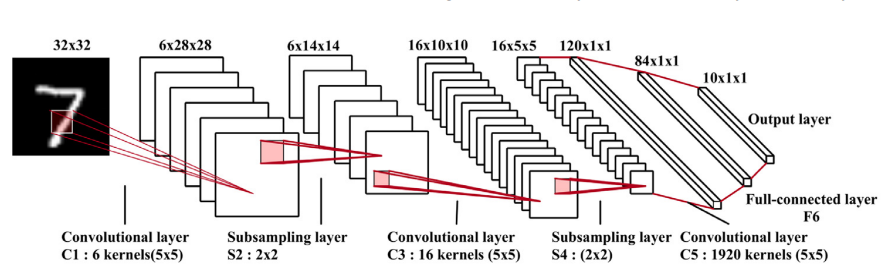
\includegraphics[width=\linewidth]{LeNet-5.png}
    \caption{LeNet-5 \cite{b6}.}
    \label{figLeNet}
\end{figure}

\begin{figure}[h]
    \centering
    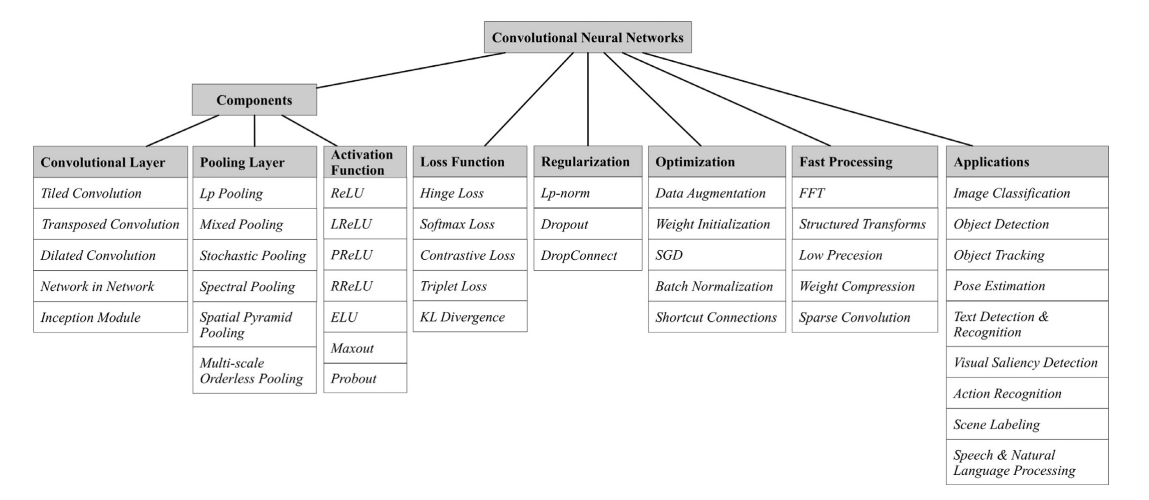
\includegraphics[width=\linewidth]{CNN_Components.png}
    \caption{Convolutional Neural Network \cite{b6}.}
    \label{figCNN}
\end{figure}

CNNs are deep neural networks that are often used for image analysis.  It can recognise images, classify them, detect objects, and identify faces. CNN comprises of neurons with learnable weights and biases. Neurons may process several inputs by creating a point as a product and possibly following it with nonlinearity. The network still expresses a single scoring function, distinguishing between raw picture pixels and class scores.  CNN provides computational efficiency through convolution, spatial integration, and parameter sharing. Thus, it enables CNN models to operate on any platform, even mobile devices \cite{b26}. Being utilized in clinical research for medical image analysis, with a strong emphasis on the clinical aspects of the field \cite{b25} along with face recognition, action recognition, image classification and natural language processing \cite{b24}.

Deep learning is a recent trend in machine learning and artificial intelligence research \cite{b27}. Many notable advancements have occurred in this sector across the world. Such studies include deep learning that can be used as an automatic system for plant counting \cite{b28}\cite{b29}.

\section{Technologies used}

\subsection{Python}

Python is used by many AI developers all around the world \cite{b8}. The reason for this is that Python plays a major role as a tool for scientific computing \cite{b8}. Reference \cite{b8} stated that the reason for Python's popularity for AI is for the following reasons:

\subsubsection{Easy to use}

Python, with its fast learning curve and easy to use syntax, is ideal for new data scientists, offering numerous data mining tools such as Rapid Miner, Weka, and Orange, and boasting significant libraries like Pandas, NumPy, SciPy, and TensorFlow, which are essential for proficient data handling and analysis \cite{b8}.

\subsubsection{Python is flexible}

Python not only allows for software creation but also facilitates numeric and logical data analysis, computing, and web development, becoming prevalent on the web by powering numerous prominent websites with frameworks like TurboGears, Django, and Tornado, making it ideal for developers skilled in application and web development \cite{b8}.

\begin{figure}[h]
    \centering
    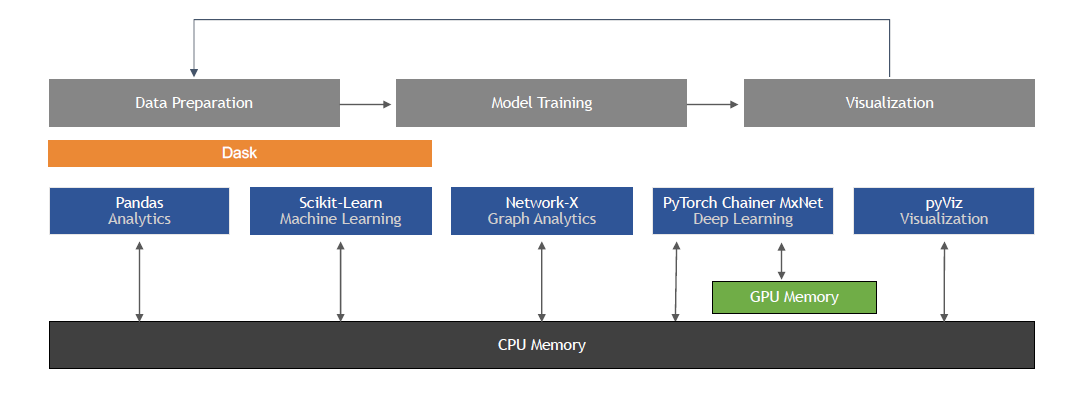
\includegraphics[width=\linewidth]{Ecosystem.png}
    \caption{The standard Python ecosystem for machine learning, data science,
    and scientific computing by \cite{b33}.}
    \label{figPY}
\end{figure}

\subsubsection{Builds better analytics tools}

Data analytics, a crucial aspect of data science, involves tools that provide insights into various frameworks, and Python is the optimal programming language for developing these tools, as it can efficiently extract knowledge, generate examples, and correlate data from large datasets, as well as support self-service analytics and assist data mining organisations in better managing their data \cite{b8}.

\subsubsection{Significant for deep learning}

Python, with its extensive packages like TensorFlow, Keras, and Theano, greatly assists data scientists in developing deep learning algorithms, which are inspired by the architecture of the human brain and involve building artificial neural networks (ANN) that simulate brain behavior by assigning weights and biases to various input parameters to produce the desired output \cite{b8}.

\subsubsection{Has a huge community base}

Python boasts a vast community of engineers and data scientists on platforms like Python.org, Fullstackpython.com, and Realpython.com, where developers can share issues and ideas, while the Python Package Index serves as an excellent resource for exploring the language's capabilities \cite{b8}.

For the reasons mentioned above Python was chosen as the programming language to create and train the model.

\subsection{PyTorch and TorchVision}

PyTorch is a Python machine learning library that shows that the 2 goals of deep learning frameworks, which are usability and speed, are compatible \cite{b9}. Popular frameworks, including Caffe, CNTK, TensorFlow, and Theano, build a static dataflow graph that represents computations, allowing for repeated application to batches of data and offering visibility into the entire computation process ahead of time \cite{b9}. While this can enhance performance and scalability, it sacrifices ease of use, ease of debugging, and flexibility in the types of computations that can be represented \cite{b9}. PyTorch that executes dynamic tensor computations with automatic differentiation and GPU acceleration immediately, maintaining performance comparable to the fastest deep learning libraries \cite{b9}.

TorchVision is a package that is available in the PyTorch library. This package consists out of various datasets, pre-trained models, and image processing tools and techniques \cite{b10}. We choose TorchVision of its image processing tools and techniques.

PyTorch was chosen since it is easier to understand than TensorFlow. TorchVision is an image processing package that is part of the PyTorch library, and for this reason TorchVision was chosen.

\subsection{Matplotlib and NumPy}

Matplotlib is a Python plotting library \cite{b8}. With Matplotlib you can write a single script that parses and plots the data, with flexibility and consistently using the Python programming language \cite{b12}. Matplotlib was modeled after MATLAB due to MATLAB's strong graphing capabilities, and the high degree of compatibility between the two led many users to transition from MATLAB to Matplotlib, making them feel at home with the latter \cite{b12}.

NumPy is a numerical Python library \cite{b8}. Since data analysis often involves operations being performed on large lists of data \cite{b8}. NumPy is a powerful tool to work quickly and easily with these data lists \cite{b8}. NumPy arrays can be treated the same as individual floats and integers, and by preforming boolean operations it is quicker to filter NumPy arrays \cite{b8}.

NumPy was used to read the images in the datasets to be read into an array and to manipulate the array, and for this reason NumPy was chosen. Matplotlib was chosen to visuale represent the batches and the size of the batches.

\subsection{Kivy and Tkinter}

Kivy is a Python based mobile application framework, that is easy to understand and user-friendly \cite{b13}. By making use of the OpenGL library feature, the Kivy framework is able to make cross-platform application development tool \cite{b13}. The Kv language separates the interface design from the application logic \cite{b14}. This allows the application to remain in Python, but the design is in the Kv language \cite{b14}. The Kivy framework is used in the mobile application to display the graphical user interface (GUI).

Tkinter is a framework that is build into the standard library of Python \cite{b15}. The Tkinter framework is only used by the mobile application so that the user can set the file path where the picture that must be analysed by the model.

Kivy was chosen as the mobile application framework for its ease of understanding and for being user-friendly. Tkinter was chosen since it is build into the standard library of Python \cite{b15}, and you can not possible to choose a file path in Kivy.

\subsection{Google Colaboratory}

Google Colaboratory, also known as Google Colab, was made by Google and is an online framework for writing, and executing Deep Learning and Machine Learning code \cite{b16}. If a researcher does not have the resources or funding for a graphics processing unit (GPU), Google Colab provides a GPU for the researcher \cite{b16}. After mounting Google Drive onto Google Colab, it can either use as a Jupyter Notebook to write and run code directly in the cells or execute Python files stored in Google Drive from the Colab environment, similar to running them from a Linux terminal, by prefixing the command with a '!' \cite{b16}. Studies have indicated that Google Colab's hardware resources can achieve performance comparable to that of dedicated hardware \cite{b17}.

Google Colab was used since the GPU, that is available on Google Colab, is more powerful than the GPU that is included in our laptops.

\section{Dataset and Preprocessing}

The dataset that was used for training this AI model was propagated at https://www.kaggle.com/datasets/sriramr/fruits-fresh-and-rotten-for-classification.

The dataset consists out of a total of 13599 photos, this includes both the testing and trained sets. Each set consists out of 6 classes that are as follows: Fresh Apples, Fresh Bananas, Fresh Oranges, Rotten Apples, Rotten Bananas, and Rotten Oranges. The training set contains a total of 10901 photos and the testing set contains a total of 2698 photos.

The photos in the training set is divided between the 6 classes as follows: Fresh Apples contains 1693 photos, Fresh Bananas contains 1591 photos, Fresh Oranges contains 1466 photos, Rotten Apples contains 2342 photos, Rotten Bananas contains 2224 photos, and Rotten Oranges contains 1595 photos.

The photos in the testing set is divided between the 6 classes as follows: Fresh Apples contains 365 photos, Fresh Bananas contains 381 photos, Fresh Oranges contains 388 photos, Rotten Apples contains 601 photos, Rotten Bananas contains 530 photos, and Rotten Oranges contains 403 photos.

The uneven distribution of the photos between the 6 classes can lead to the model falsely identify the class that a test photo belong to.

\begin{figure}[h]
    \centering
    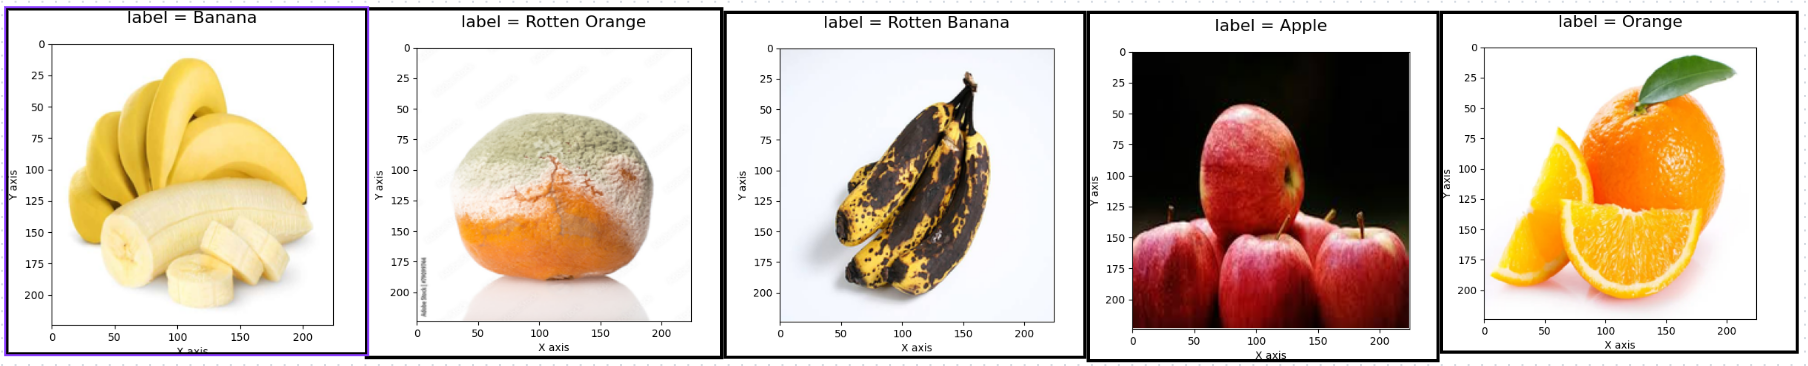
\includegraphics[width=\linewidth]{Example_data.png}
    \caption{Example dataset.}
    \label{fig}
\end{figure}

For the training dataset, the images are preprocessed through several steps. First, they are resized to a fixed size of 224x224 pixels. Then, random horizontal flipping is applied, which is a data augmentation technique to increase the diversity of training data. Next, the images are converted to PyTorch tensors, scaling the pixel values to the range [0, 1]. Finally, the images are normalised by subtracting the mean values [0.485, 0.456, 0.409] from each color channel (RGB) and dividing by the standard deviations [0.229, 0.224, 0.225].

For the test dataset, the preprocessing steps are similar but without the random horizontal flipping step. The images are resized to 224x224 pixels, converted to PyTorch tensors with pixel values scaled to [0, 1], and normalised using the same mean and standard deviation values as the training dataset. Consistent preprocessing between the training and test data is essential for accurate model evaluation and inference.

Automatic image colorisation adds colours to grayscale images without user intervention \cite{b11}. Many methods allow users to specify colours for certain areas, which are then extended to the entire image \cite{b11}. This extension can be achieved by segmenting the image into homogeneous colour regions or by spreading colours from user-defined points \cite{b11}. The spread of colour is often guided by local grayscale intensity variations or a predefined threshold to detect colour edges \cite{b11}. Fig. \ref{fig1} shows how the colorisation is done on an image that is input into the mobile application.

\begin{figure}[h]
    \centering
    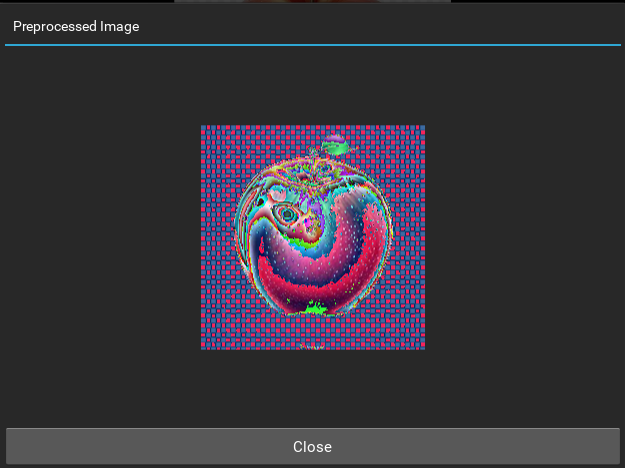
\includegraphics[width=\linewidth]{Pre-pros_image.png}
    \caption{Example of Colorisation.}
    \label{fig1}
\end{figure}

\section{Model Architecture}

The model makes use of structured learning during the training phase. Structured learning makes use of labels to train a model to preform classification tasks \cite{b1}. The labels used in this model are as follows: freshapples, freshbanana, freshoranges, rottenapples, rottenbanana, and rottenoranges.

The architecture of the model, as seen in Fig. \ref{fig2}, is as follows:
\begin{itemize}
    \item Input layer: Takes an input image of size (3, H, W), where 3 represents the RGB.
    \item Conv2d layers: Each convolutional layer is followed by a BatchNorm2d and ReLU activation.
    \item Dropout layer: Applied to avoid overfitting.
    \item Fully connected layers: the first linear layer reduces the flattened features, followed by a ReLU activation, and the second linear layer maps the features to the 6 output classes.
    \item Output layer: Provides the classification output for the 6 classes.
\end{itemize}

\begin{figure}[h]
    \centering
    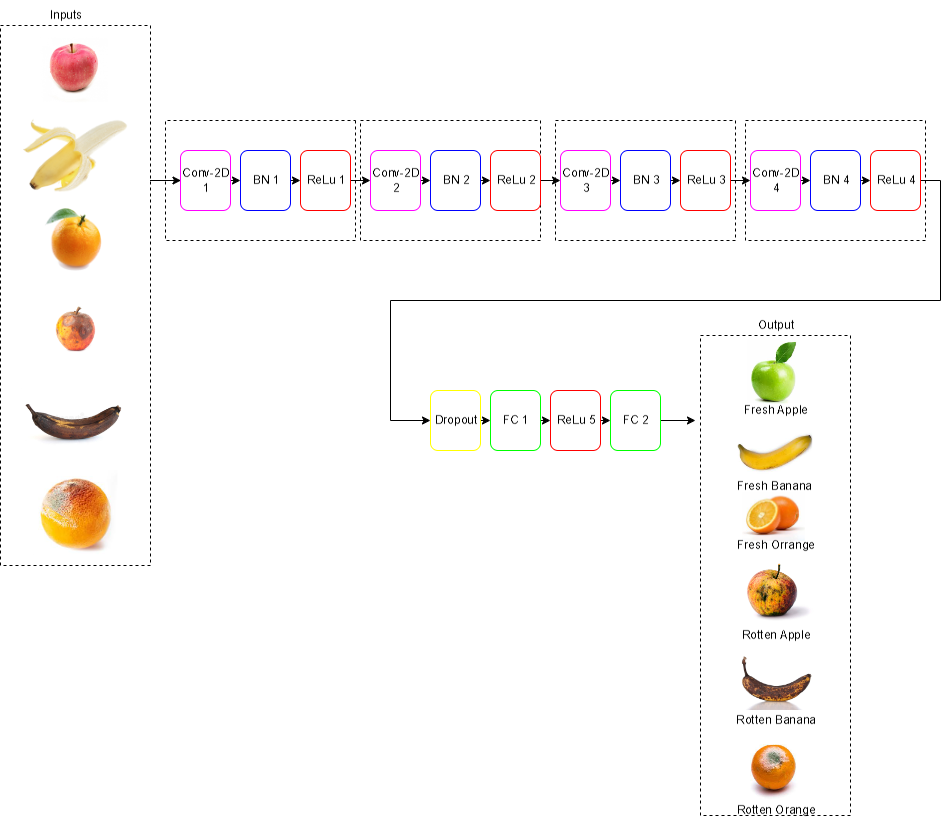
\includegraphics[width=\linewidth]{Ai_Prent.drawio_1_1.png}
    \caption{Neural Network Architecture.}
    \label{fig2}
\end{figure}

\section{Rectified Linear Unit (ReLU)}

Rectified Linear Unit (ReLU) can be effectively used in both pre-training and classification and is widely used in many applications \cite{b7}. The structure of a deep network is complex, so it is hard to analyse the dynamics of learning process thus, we study how complex networks need to be to approximate certain functions \cite{b7}. In this process, we optimize the trade-off between neural network complexity (measured by nonzero weights) and approximation fidelity for piecewise constant (or piecewise smooth) functions \cite{b7}.
\begin{figure}[h]
    \centering
    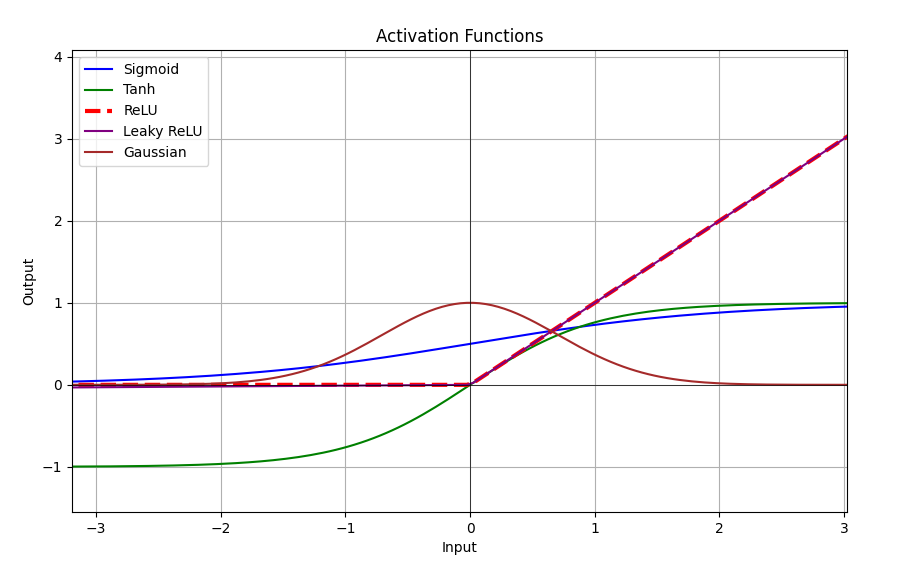
\includegraphics[width=\linewidth]{Activation_Functions_Compare.PNG}
    \caption{Activation Functions Comparison}
    \label{fig}
\end{figure}
\\
\\
The function is defined as
\[f(x) = x^{\ +\ } = \max(0,x) = \frac{x+|x|}{2} = \begin{cases}
    x & \text{if } x > 0 \\
    0 & \text{otherwise}
\end{cases}
\]

\subsection{ReLU over Sigmoid}

Being computationally simple and efficient compared to other activation functions like sigmoid and tanh \cite{b30}. Which means it requires only a thresholding at zero\cite{b30}. This simplicity reduces the computational overhead during both the forward and backward passes of the network, speeding up the training process \cite{b30}.

ReLU does not saturate in the positive domain. Unlike sigmoid or tanh, which can suffer from vanishing gradients due to their output being bounded between 0 and 1 or -1 and 1 respectively, ReLU outputs raw positive values \cite{b30}. This helps in maintaining a strong gradient flow, especially in deeper networks, which facilitates faster convergence \cite{b31}.

ReLU introduces sparsity by outputting zero for any input less than zero \cite{b31}. This sparsity means that neurons are only activated for a subset of inputs, leading to a more efficient representation and reducing the risk of overfitting \cite{b31}. Sparse activations also reduce the interdependence of neurons, making the model less likely to suffer from redundancy \cite{b31}.

ReLU is more biologically plausible compared to functions like sigmoid and tanh \cite{b30}. It is similar to the firing rate of biological neurons, which are either active (firing) or inactive (not firing), rather than outputting a continuous range of values \cite{b31}.

ReLU has been empirically shown to perform well across a wide range of tasks and architectures \cite{b32}. Many deep learning models that achieve results in areas such as image recognition, natural language processing, and reinforcement learning use ReLU as the activation function \cite{b32}.

While sigmoid and tanh suffer from the vanishing gradient problem where gradients can become extremely small during backpropagation, leading to slow learning or even stagnation, ReLU helps mitigate this issue \cite{b30}. In the positive range, the gradient of ReLU is always one, which helps maintain gradient magnitude \cite{b30}.

\section{Training Process}

The process of training the model went through different iterations.

With the first iteration we only had 1 convolutional layer with a batch size of 128 and the training was done on the CPU. This caused that the model would take longer to train, and the model was not accurate with classifying the if fruit are fresh or rotten. During the second iteration the model still had 1 convolutional layer, but we lessened the batch size to 64 and the training was moved from the CPU to the GPU. A smaller batch size helps to increase the accuracy of an AI model \cite{b2} and helps prevent overfitting the model, and by moving the training from the CPU to the GPU we experienced a decrease in the time that it takes the model to train. But we still had a problem with the accuracy of the model.

The third iteration was the iteration where the amount of convolutional layers was increased from 1 to 4. This help to reduce the complexity of the model through the optimisation of each layer outputs \cite{b3}. For the forth iteration a Google Colab environment was used to train the model and the batch size was decreased to 32. By using Google Colab we were able to train the model by using a cloud base GPU. This allowed us to decrease the time that it took the model to train.

The fifth iteration was the final iteration and for this iteration we changed the amount of epochs from 50 to 150. By changing the epoch the amount of time that the model will work through the training \cite{b4}. To avoid overfitting the AI model we added a patience variable. 

\section{Experimentation and Results}

In order to create the final AI model that would is used in the application we preformed different experiments. These experiments include changing the epochs, changing the batch size, adding dropout layers, adding more convolutional layers, and adding a patience variable.

\subsection{Changing the Epochs}

With the first and second iterations of training the model the epoch was set to 20. From the third and forth iterations the epoch was set to 50. The fifth and final iteration the epoch was set to 150.

The epoch for the first and second iterations was chosen since it was the testing phase to find the best epoch for the model. For the third and forth iterations the epoch was set to 50 after reading \cite{b4} and testing, but the model was still not accurate. The final epoch for the fifth iteration was chosen since we wanted the model to train in one sitting, this was found to be the most effective epoch for training.

\subsection{Changing the Batch size}

The original batch size for training the model was 128. During the course of the iterative process of training the model the batch size was decreased to 64 and in the final iteration of training the model the batch size was decreased to 32.

This was done to increase the accuracy of the model after training, since by decreasing the batch size meant that the model would look at more images during the training process. Fig. \ref{fig4} provides a visual representation of how one of the batches look.

\begin{figure}[h]
    \centering
    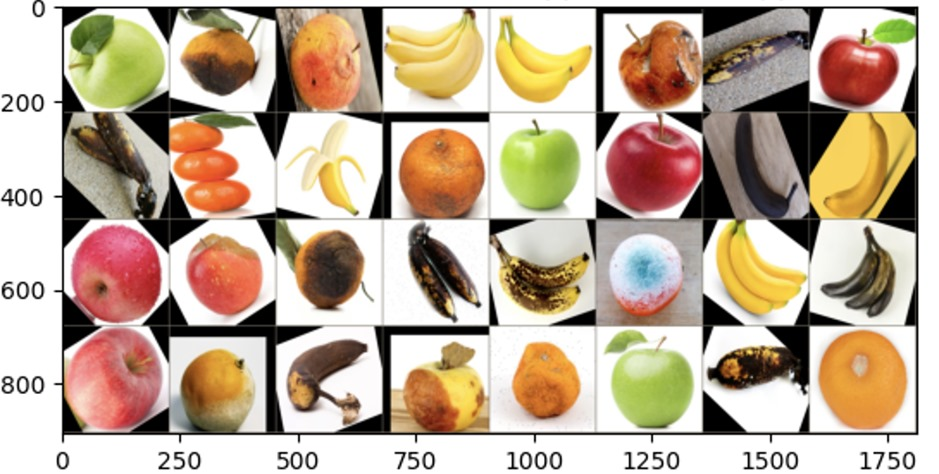
\includegraphics[width=\linewidth]{Batch_Representation.jpg}
    \caption{Visual Representation of a Batch}
    \label{fig4}
\end{figure}

\subsection{More Convolutional Layers}

During the first 2 iterations of the training process our model only had 1 convolutional layer, this was done at first only to see if it is possible to create and train our own model. 

The third iteration was the first iteration where more layers were added. In this iteration the amount of convolutional layers went form 1 to 4 layers, this was done to increase the accuracy of the model by reducing the complexity of the convolutional network \cite{b3}.

\subsection{Adding Dropout Layers}

Before the third iteration of the training process, the model did not have a dropout layer. The dropout layer was only added in the third iteration of the training process.

The dropout layer was added to avoid overfitting the model. The dropout layer works by removing neurons from the network based on their activation \cite{b5}. If the activation of a neuron in the network is greater than our dropout value, which is 0.5, the likelihood of deactivating the neuron is increased.

\subsection{Adding a Patience Variable}

Since the epoch for the training of the model was 50 or less we did not add a patience variable, but since with the fifth and final iteration with the epoch set to 150 it was needed to add a patience variable, to ensure that once the model reached a state where there was no longer any improvement the model would stop training.

The patience variable for the training of the model was set to 10. And to measure if the model was improving we added a loss function. The loss was calculated by dividing the running loss of the epoch by the size of the train dataset. The lower the loss value the more accurate the model is, and this value's model is saved as the best loss value. In order for the patience variable to take effect the best loss value would have to be the same for 10 epochs. If the best loss value stayed the same for the 10 epochs the model would stop training. Since if the model would continue training after no impairments where made there would be a chance that the model could be overfitted \cite{b5}. Fig. \ref{fig5} shows how the loss value decreased with each epoch.

\begin{figure}[h]
    \centering
    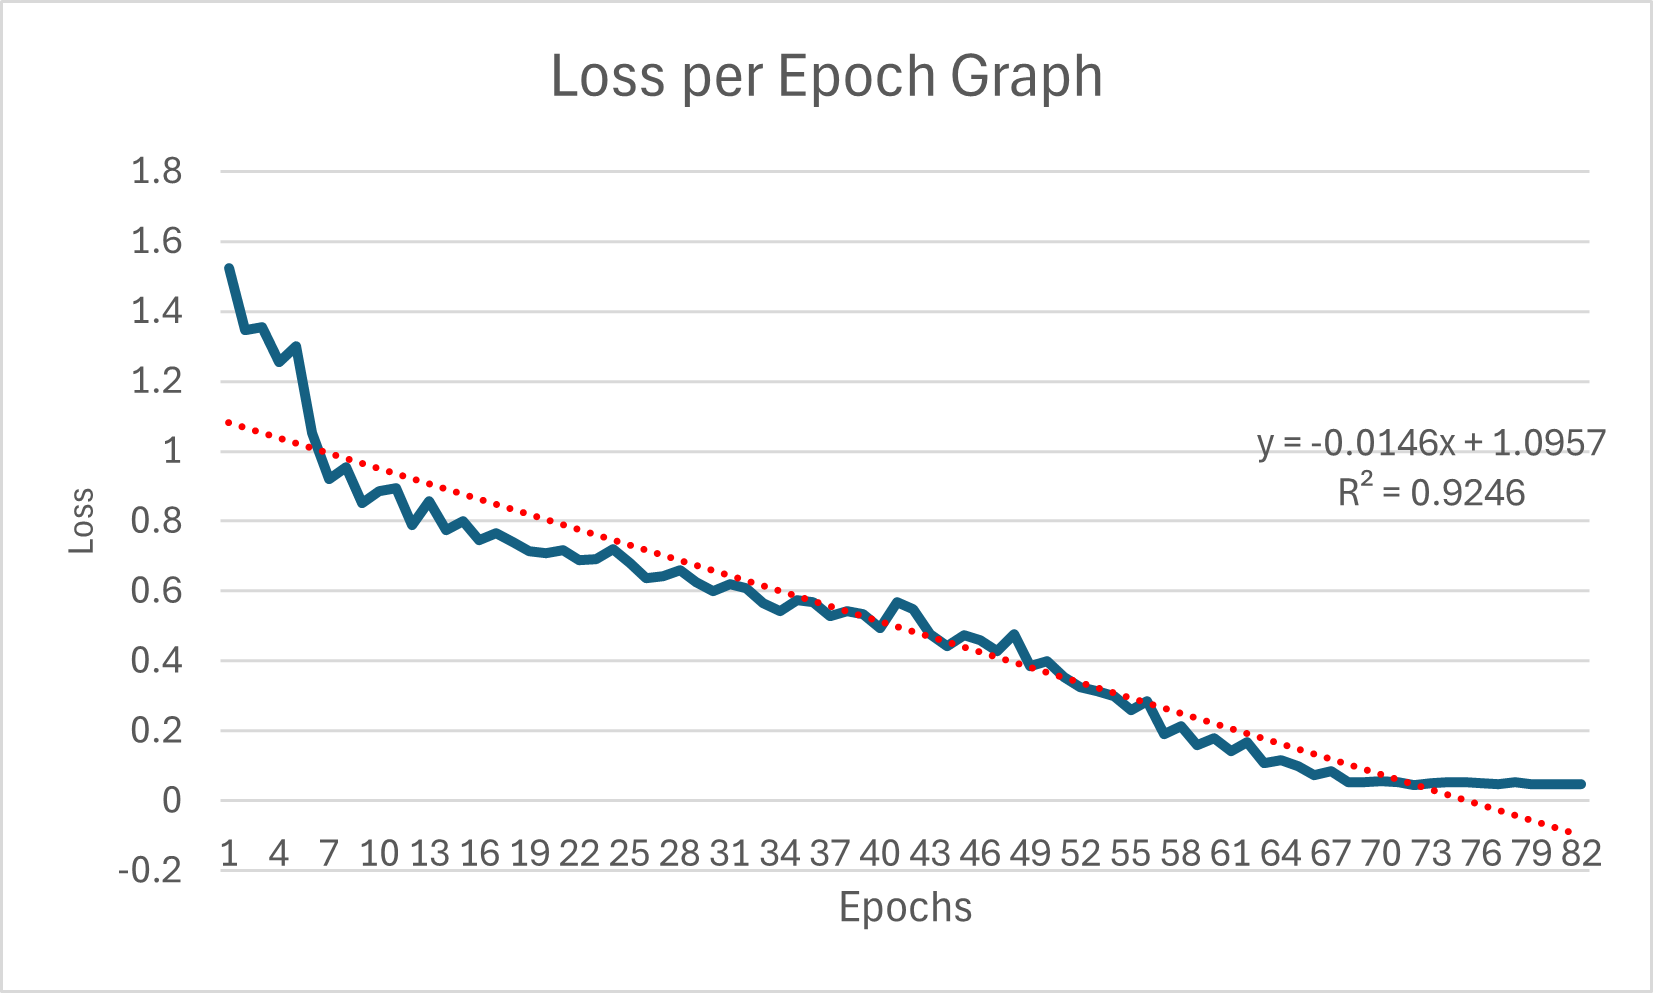
\includegraphics[width=\linewidth]{Loss_per_Epoch_Graph.png}
    \caption{Loss per Epoch.}
    \label{fig5}
\end{figure}

\subsection{Learning Rate}
The learning rate for the fruit freshness detection AI model was 0.001. The reason for chosen this learning rate for the model is because the optimal learning rate must be between 0.01 and 0.001 \cite{b34}.

\section{Shortcomings of the Model}

Although the model can correctly classifying fruits that are part of the dataset that the model has been trained on, with an accuracy of 0.981. The model still has shortcomings. In this section some identified shortcomings will be discused. 

\subsection{Limited data}

In nature there are different variants of fruits, such as a red banana \cite{b18}. Fig. \ref{FigLimDataV} shows that the model falsely classify different variants. The reason why this occurs is that the Kaggle dataset used for training does not include the different variants of apples, bananas, and oranges. For the model to correctly classify these variants of the fruits, they need to be included in the dataset.

\begin{figure}[h]
    \centering
    \begin{subfigure}[b]{0.48\linewidth}
        \centering
        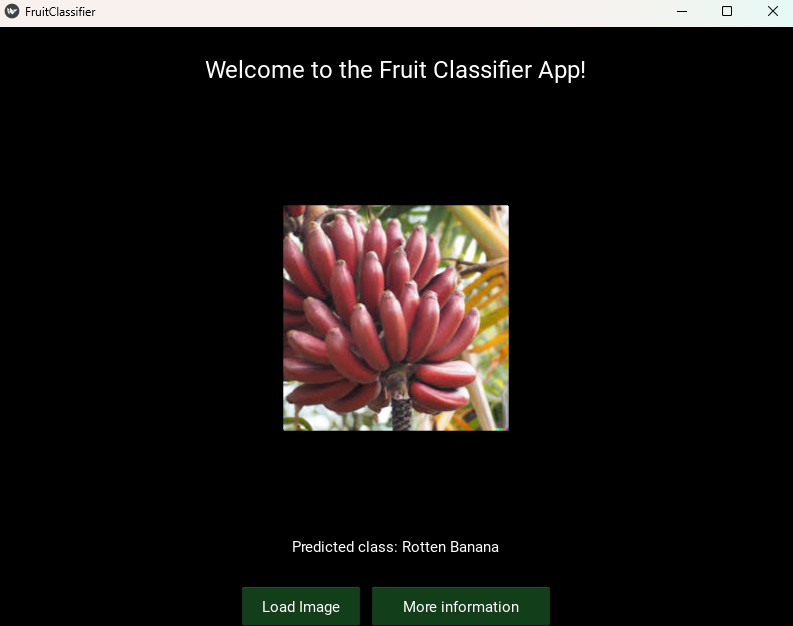
\includegraphics[width=\linewidth]{Red Banana not seen as banana.png}
        \caption{Flase Classification.}
        \label{figFA}
    \end{subfigure}
    \hfill
    \begin{subfigure}[b]{0.48\linewidth}
        \centering
        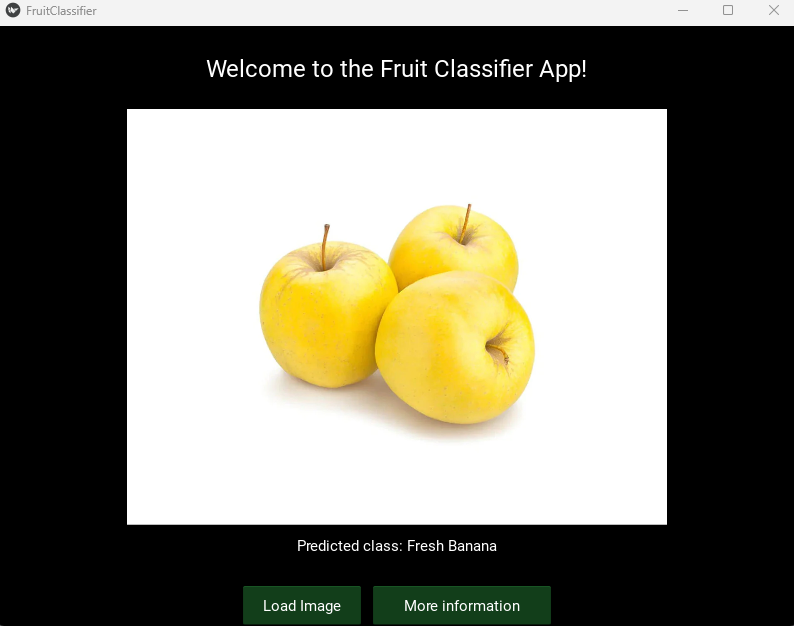
\includegraphics[width=\linewidth]{Yellow Apples not seen as apples.png}
        \caption{False Classification.}
        \label{figFB}
    \end{subfigure}
    \caption{False classification due to Limited Data.}
    \label{FigLimDataV}
\end{figure}

The current model in only trained to classify if an apple, banana, or orange are either fresh or rotten. Fig. \ref{FigLimData} shows what that model can not correctly fruit that are not part of the train dataset. In order for the model to correctly classify these fruits they would have to be added to the dataset, and a class for these fruits will have to be added to the model for both fresh and rotten.

\begin{figure}[h]
    \centering
    \begin{subfigure}[b]{0.48\linewidth}
        \centering
        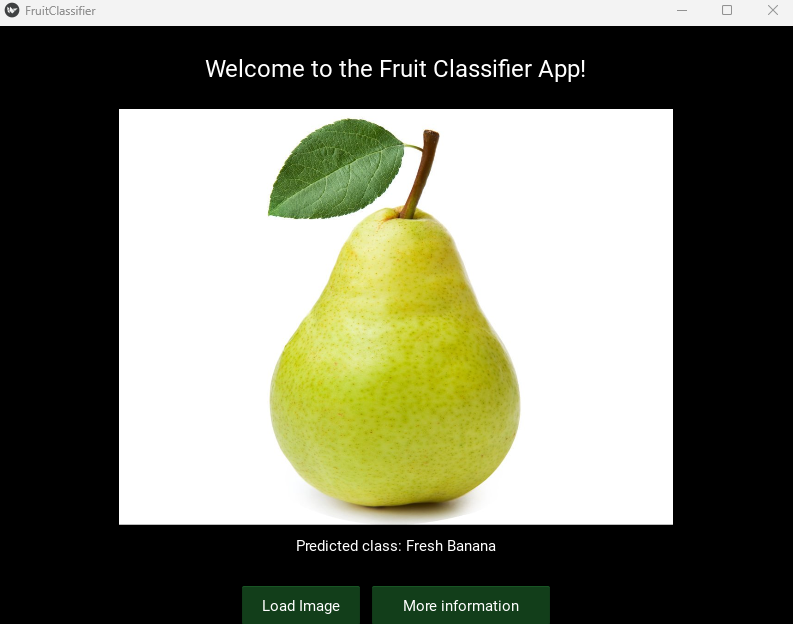
\includegraphics[width=\linewidth]{Pear not in dataset.png}
        \caption{Flase Classification.}
        \label{figFA}
    \end{subfigure}
    \hfill
    \begin{subfigure}[b]{0.48\linewidth}
        \centering
        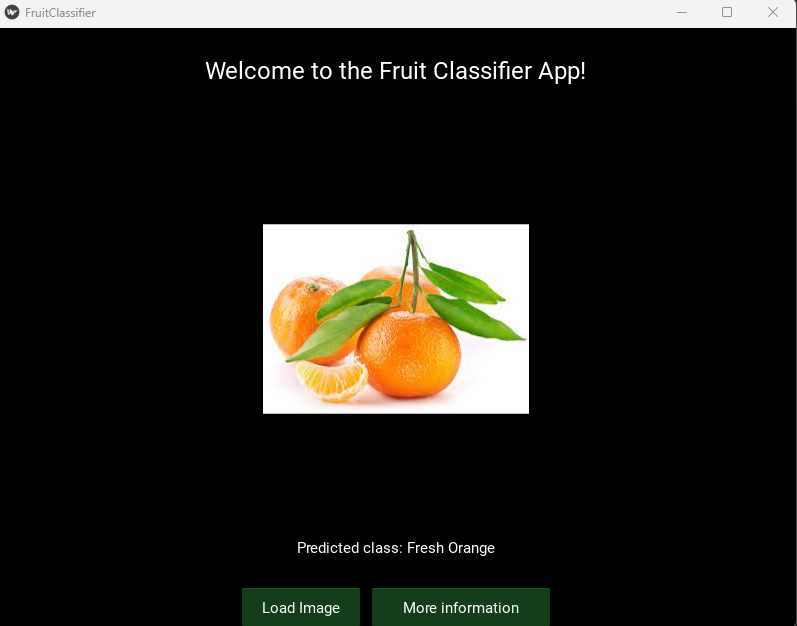
\includegraphics[width=\linewidth]{Tangerine not in dataset.png}
        \caption{False Classification.}
        \label{figFB}
    \end{subfigure}
    \caption{False Classification due to Limited Data.}
    \label{FigLimData}
\end{figure}

\subsection{Noise in Image}

In images, noise refers to random variations in brightness or color that degrade image quality, making it appear grainy or speckled, and can arise from various sources \cite{b19}. Common types of noise include Gaussian noise from sensor electronics, salt-and-pepper noise from signal disturbances, and Poisson noise from low light conditions \cite{b19}. By making use of edge detection to mark out the edges of the fruit \cite{b20}, this can help the model to accurately identify the class that the fruit belongs to, Fig. \ref{FigNoise} shows the result of an image wit noise and the result after edge detection have been implemented.

\begin{figure}[h]
    \centering
    \begin{subfigure}[b]{0.48\linewidth}
        \centering
        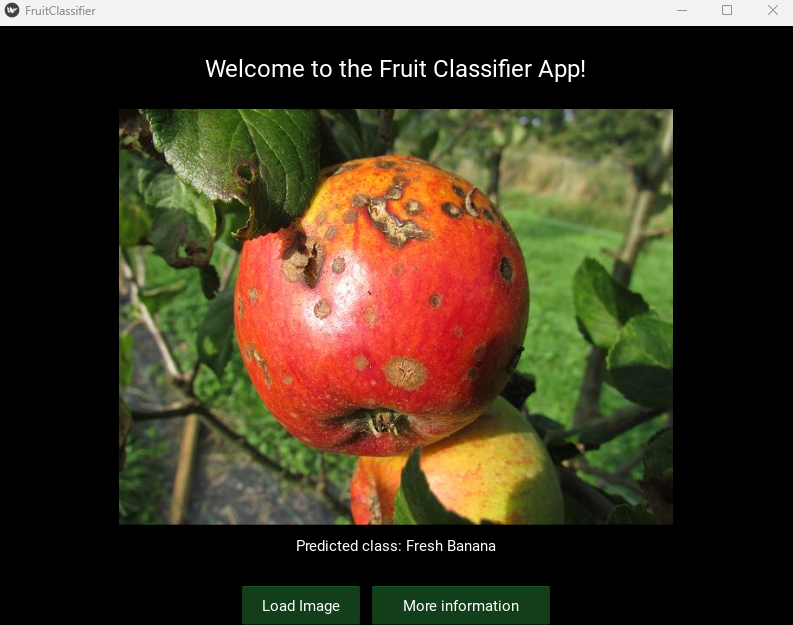
\includegraphics[width=\linewidth]{Apple with noise.png}
        \caption{Classification with Noise.}
        \label{figFA}
    \end{subfigure}
    \hfill
    \begin{subfigure}[b]{0.48\linewidth}
        \centering
        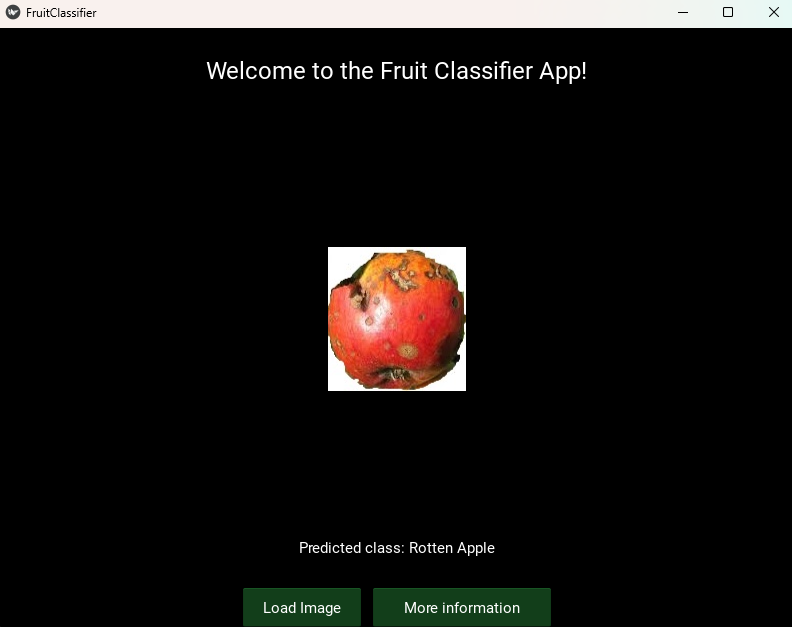
\includegraphics[width=\linewidth]{Apple processed.png}
        \caption{Classification without Noise.}
        \label{figFB}
    \end{subfigure}
    \caption{Classification with Noise and without Noise.}
    \label{FigNoise}
\end{figure}

\section{Results and Discusion}

\subsection{Single layer}

\begin{figure}[h]
    \centering
    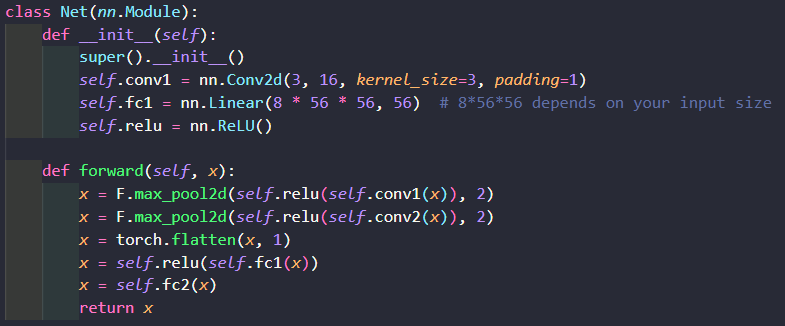
\includegraphics[width=\linewidth]{single layer arc.png}
    \caption{Single Layer Architecture.}
    \label{figSl}
\end{figure}

\begin{figure}[h]
    \centering
    \begin{subfigure}[b]{0.48\linewidth}
        \centering
        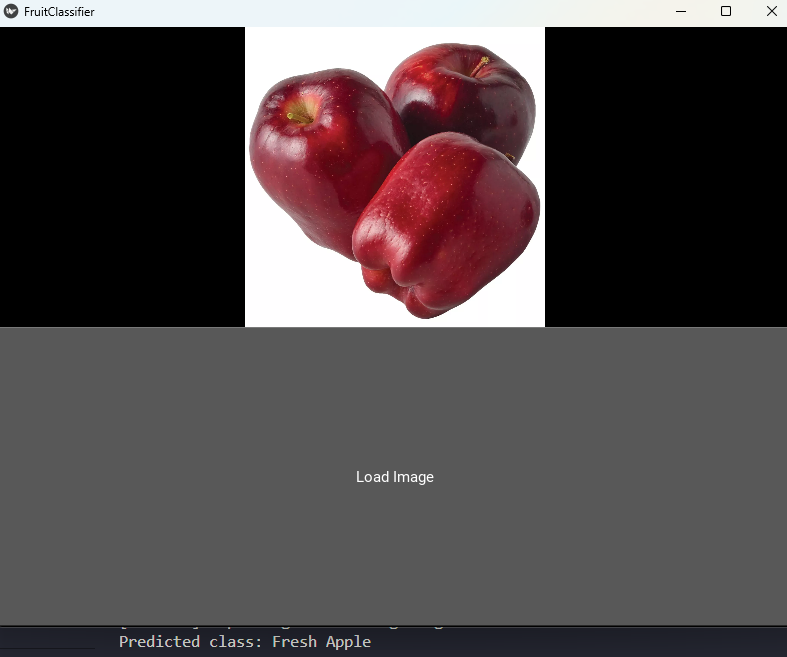
\includegraphics[width=\linewidth]{1layer appel1.png}
        \caption{First Version Apple 1 Classification.}
        \label{figFA}
    \end{subfigure}
    \hfill
    \begin{subfigure}[b]{0.48\linewidth}
        \centering
        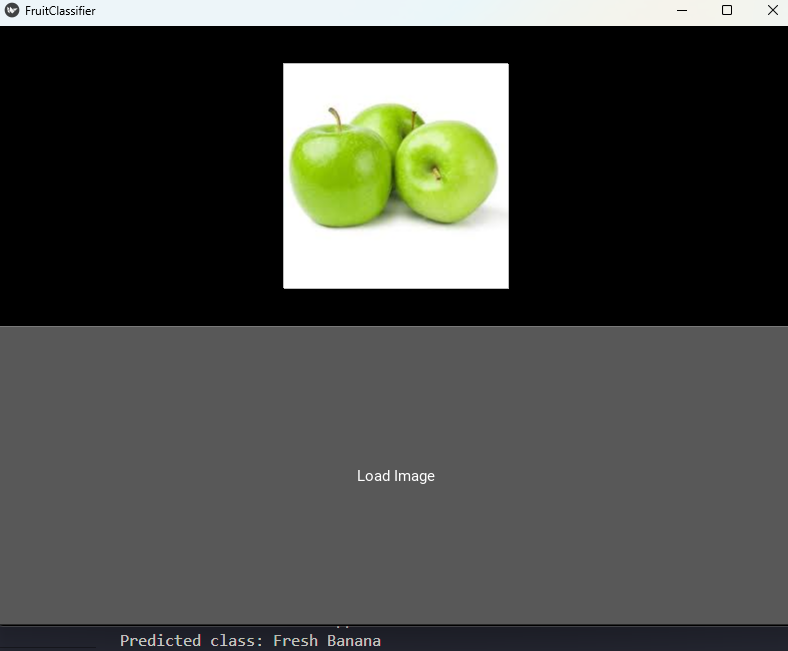
\includegraphics[width=\linewidth]{1layer appel2.png}
        \caption{First Version Apple 2 Classification.}
        \label{figFB}
    \end{subfigure}
    \hfill
    \begin{subfigure}[b]{0.48\linewidth}
        \centering
        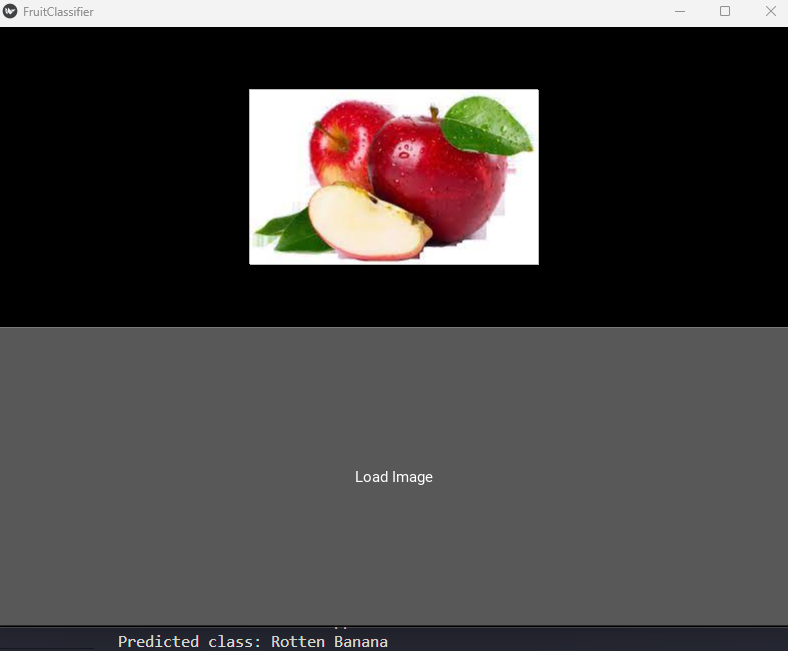
\includegraphics[width=\linewidth]{1layer appel3.png}
        \caption{First Version Apple 3 Classification.}
        \label{figFB}
    \end{subfigure}
    \hfill
    \begin{subfigure}[b]{0.48\linewidth}
        \centering
        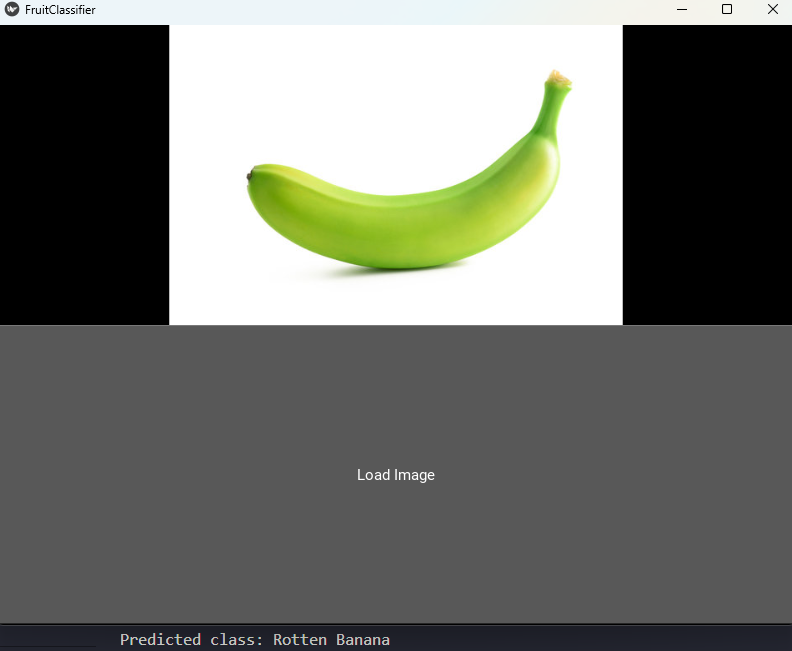
\includegraphics[width=\linewidth]{1layer banana1.png}
        \caption{First Version Banana 1 Classification.}
        \label{figFA}
    \end{subfigure}
    \hfill
    \begin{subfigure}[b]{0.48\linewidth}
        \centering
        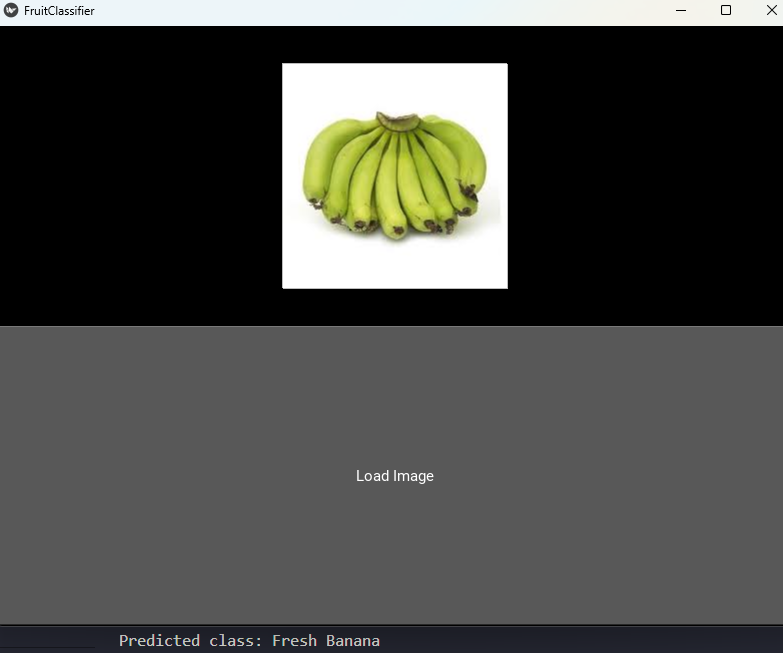
\includegraphics[width=\linewidth]{1layer banana2.png}
        \caption{First Version Banana 2 Classification.}
        \label{figFB}
    \end{subfigure}
    \hfill
    \begin{subfigure}[b]{0.48\linewidth}
        \centering
        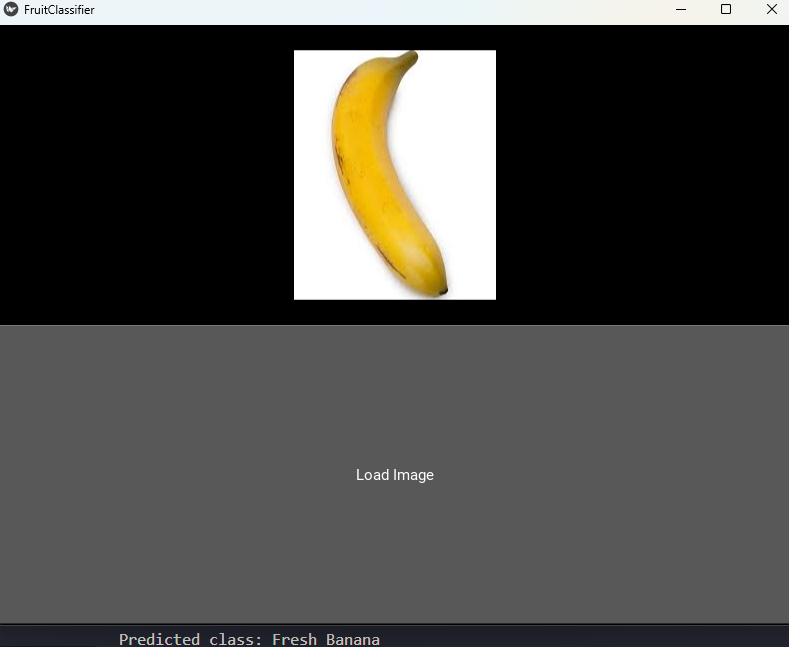
\includegraphics[width=\linewidth]{1layer banana3.png}
        \caption{First Version Banana 3 Classification.}
        \label{figFB}
    \end{subfigure}
    \hfill
    \begin{subfigure}[b]{0.48\linewidth}
        \centering
        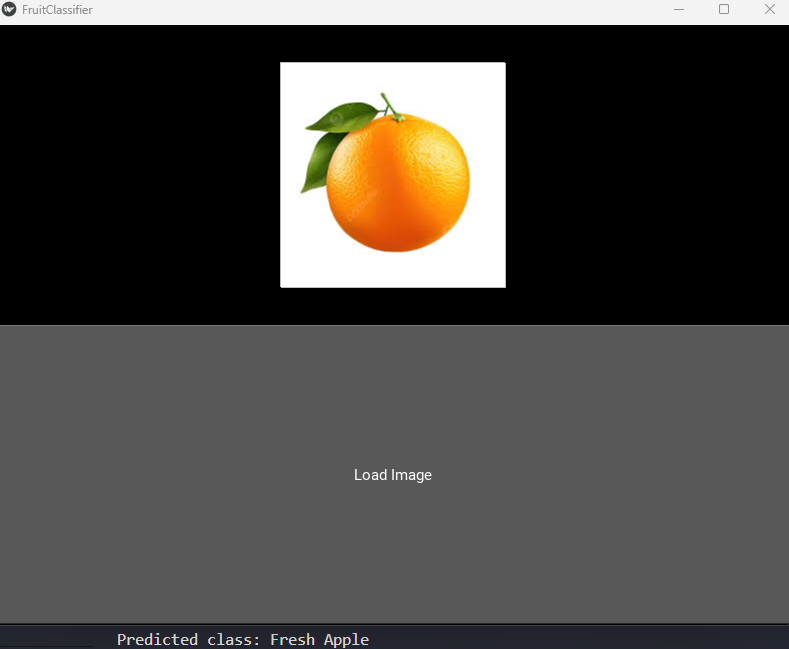
\includegraphics[width=\linewidth]{1layer orage1.png}
        \caption{First Version Orange 1 Classification.}
        \label{figFA}
    \end{subfigure}
    \hfill
    \begin{subfigure}[b]{0.48\linewidth}
        \centering
        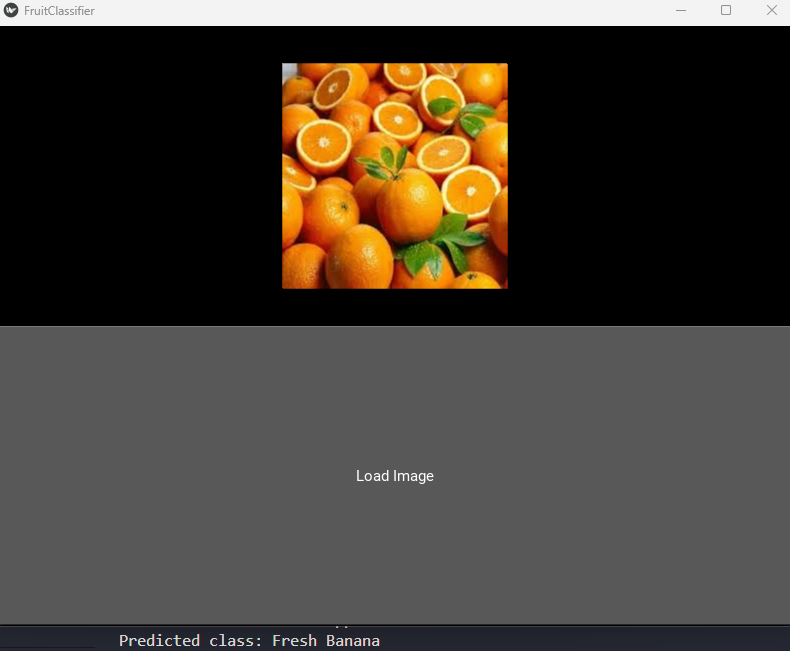
\includegraphics[width=\linewidth]{1layer orage2.png}
        \caption{First Version Orange 2 Classification.}
        \label{figFB}
    \end{subfigure}
    \hfill
    \begin{subfigure}[b]{0.48\linewidth}
        \centering
        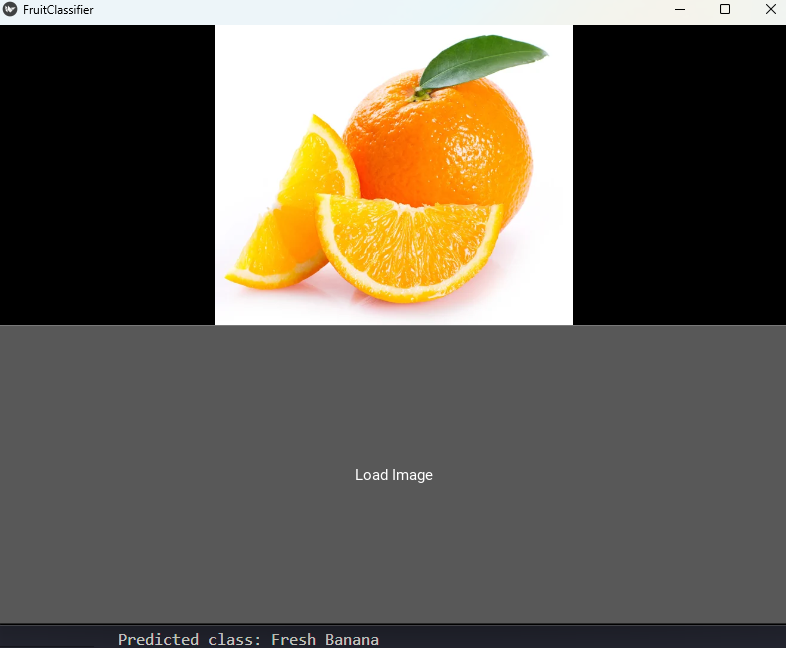
\includegraphics[width=\linewidth]{1layer orage3.png}
        \caption{First Version Orange 3 Classification.}
        \label{figFB}
    \end{subfigure}
    \caption{First Version Classification of Fresh Fruit.}
    \label{Fig1F}
\end{figure}

\begin{figure}[h]
    \centering
    \begin{subfigure}[b]{0.48\linewidth}
        \centering
        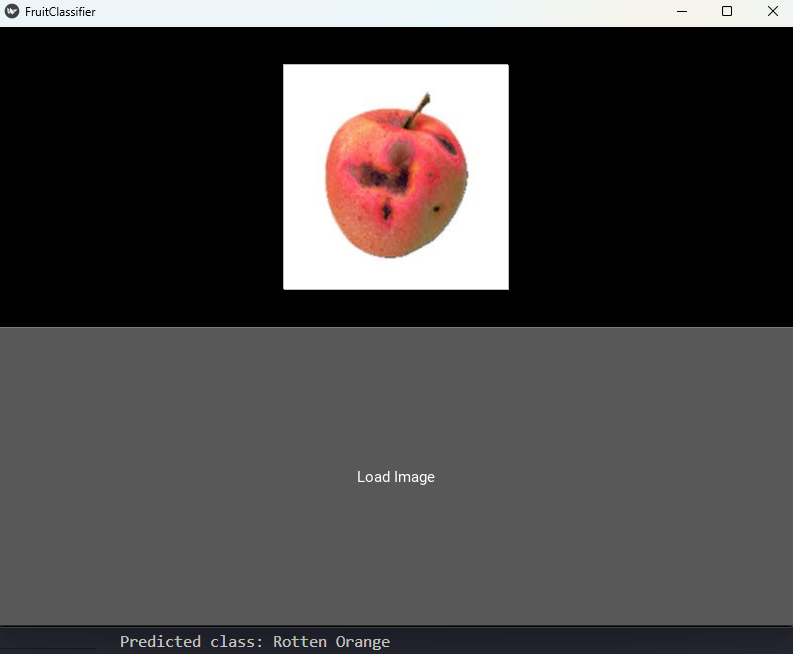
\includegraphics[width=\linewidth]{1layer appelR1.png}
        \caption{First Version Apple 1 Classification.}
        \label{figFA}
    \end{subfigure}
    \hfill
    \begin{subfigure}[b]{0.48\linewidth}
        \centering
        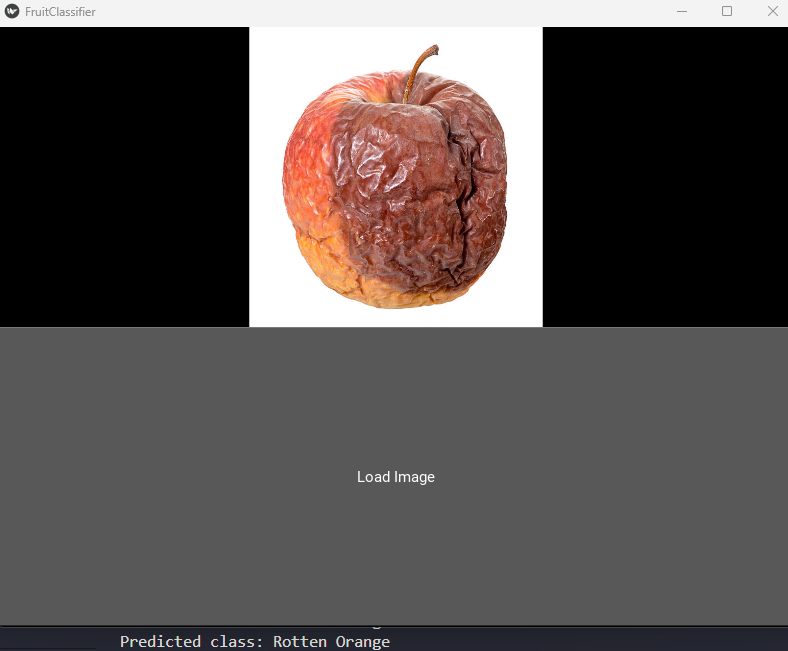
\includegraphics[width=\linewidth]{1layer appelR2.png}
        \caption{First Version Apple 2 Classification.}
        \label{figFB}
    \end{subfigure}
    \hfill
    \begin{subfigure}[b]{0.48\linewidth}
        \centering
        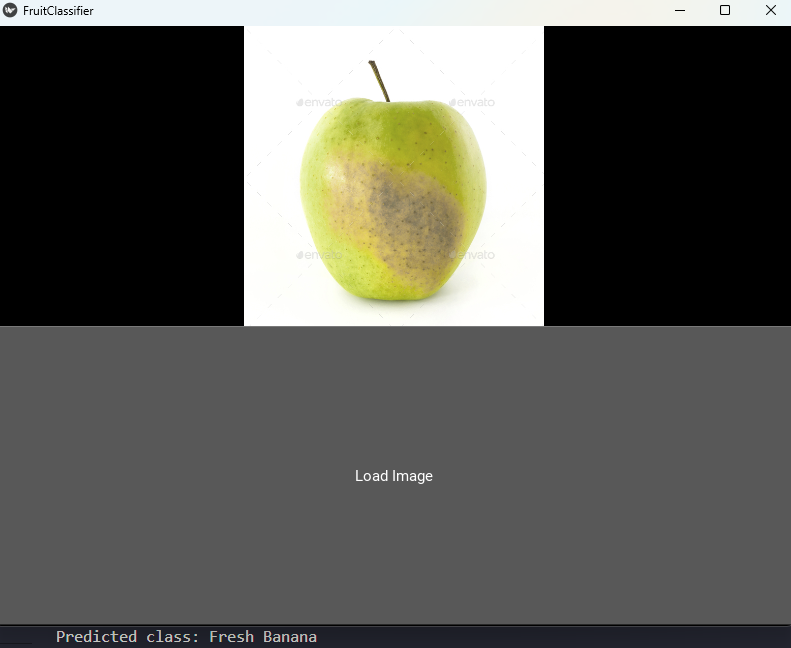
\includegraphics[width=\linewidth]{1layer appelR3.png}
        \caption{First Version Apple 3 Classification.}
        \label{figFB}
    \end{subfigure}
    \hfill
    \begin{subfigure}[b]{0.48\linewidth}
        \centering
        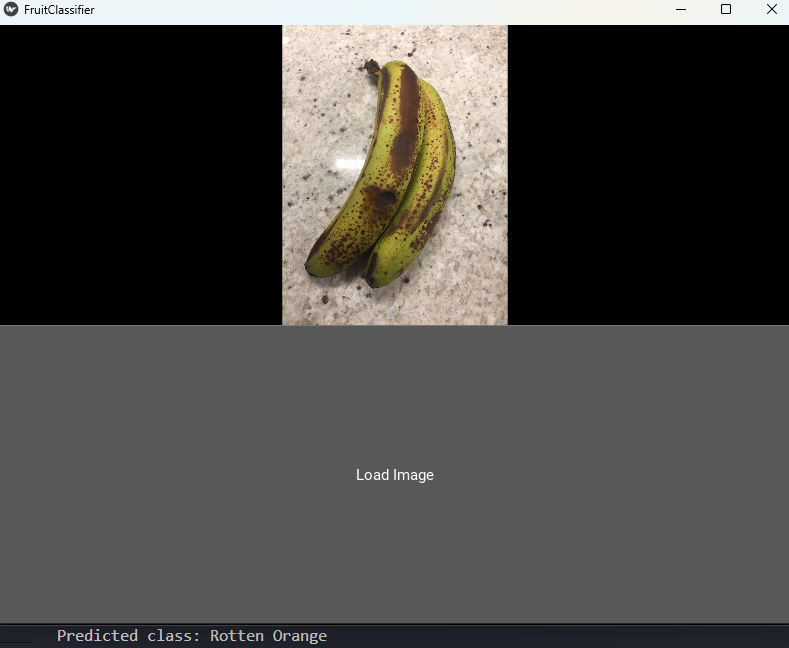
\includegraphics[width=\linewidth]{1layer bananaR1.png}
        \caption{First Version Banana 1 Classification.}
        \label{figFA}
    \end{subfigure}
    \hfill
    \begin{subfigure}[b]{0.48\linewidth}
        \centering
        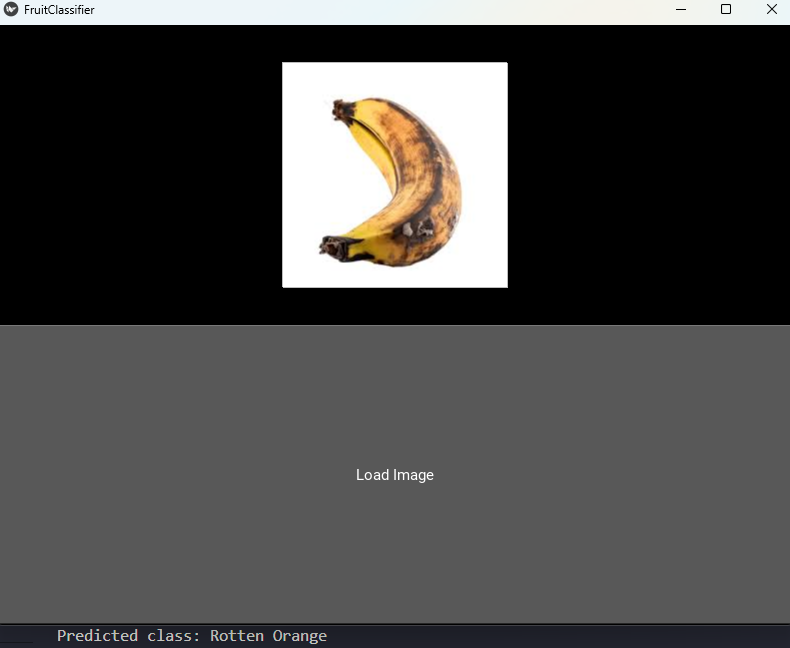
\includegraphics[width=\linewidth]{1layer bananaR2.png}
        \caption{First Version Banana 2 Classification.}
        \label{figFB}
    \end{subfigure}
    \hfill
    \begin{subfigure}[b]{0.48\linewidth}
        \centering
        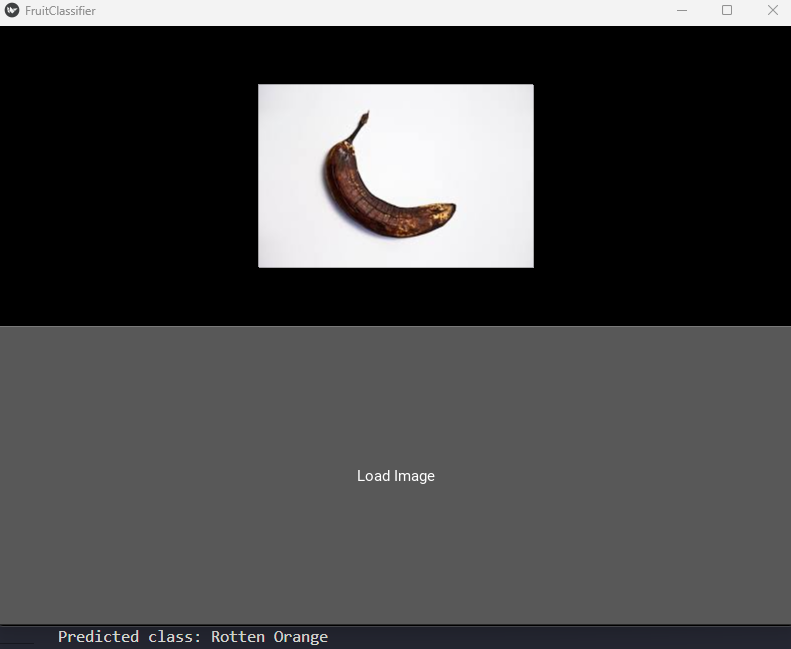
\includegraphics[width=\linewidth]{1layer bananaR3.png}
        \caption{First Version Banana 3 Classification.}
        \label{figFB}
    \end{subfigure}
    \hfill
    \begin{subfigure}[b]{0.48\linewidth}
        \centering
        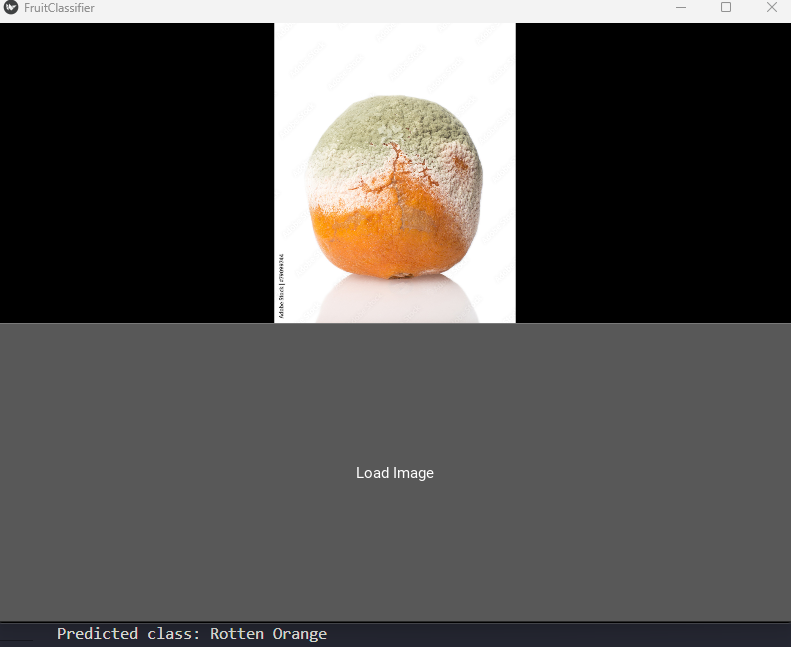
\includegraphics[width=\linewidth]{1layer orageR1.png}
        \caption{First Version Orange 1 Classification.}
        \label{figFA}
    \end{subfigure}
    \hfill
    \begin{subfigure}[b]{0.48\linewidth}
        \centering
        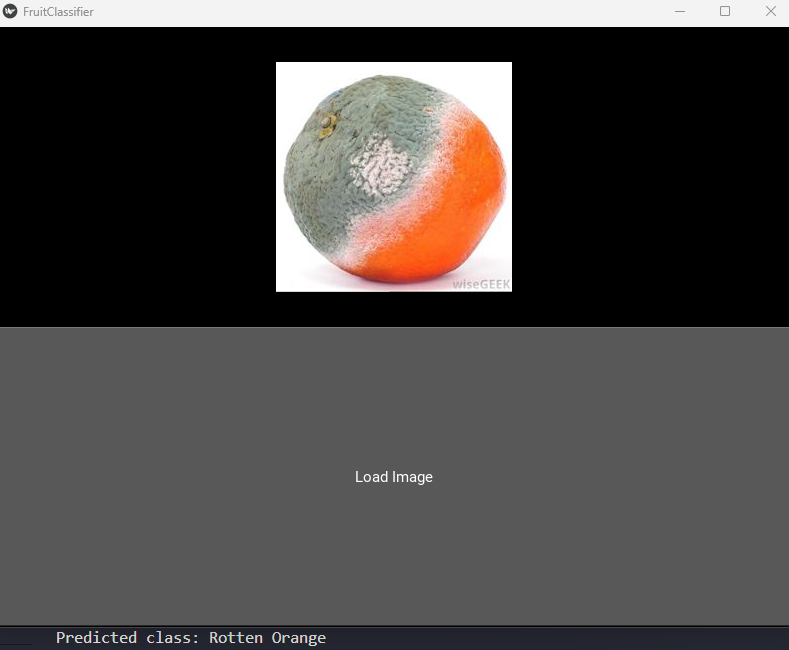
\includegraphics[width=\linewidth]{1layer orageR2.png}
        \caption{First Version Orange 2 Classification.}
        \label{figFB}
    \end{subfigure}
    \hfill
    \begin{subfigure}[b]{0.48\linewidth}
        \centering
        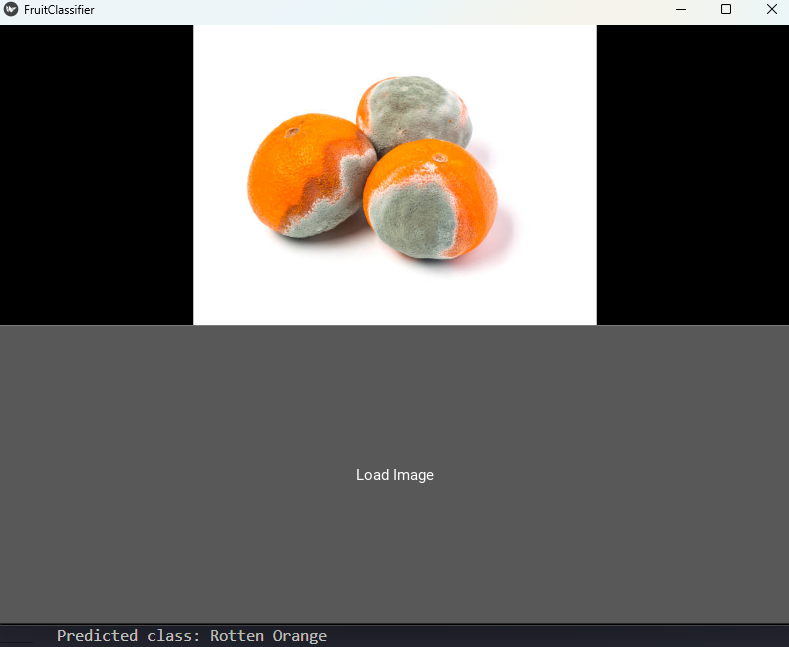
\includegraphics[width=\linewidth]{1layer orageR3.png}
        \caption{First Version Orange 3 Classification.}
        \label{figFB}
    \end{subfigure}
    \caption{First Version Classification of Rotten Fruit.}
    \label{Fig1R}
\end{figure}
\clearpage

\subsection{Multi layer}

\begin{figure}[h]
    \centering
    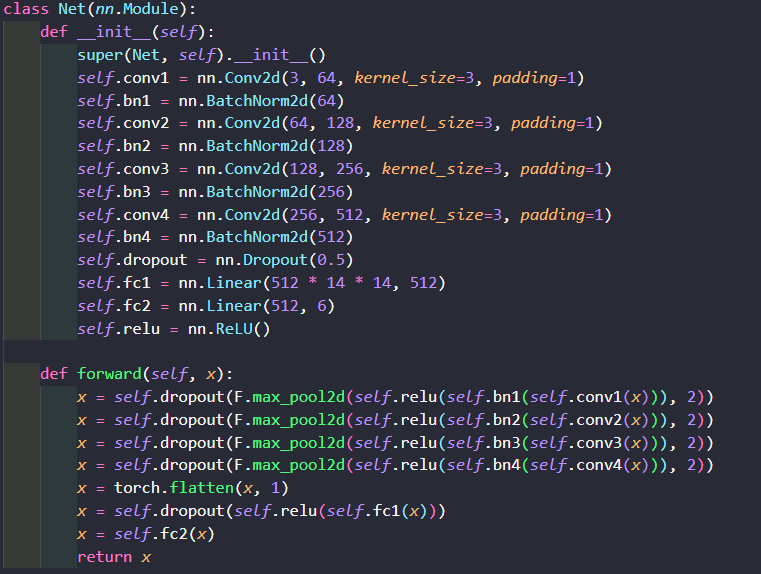
\includegraphics[width=\linewidth]{multi architecture.png}
    \caption{Multi Layer Architecture.}
    \label{figMl}
\end{figure}

\begin{figure}[h]
    \centering
    \begin{subfigure}[b]{0.48\linewidth}
        \centering
        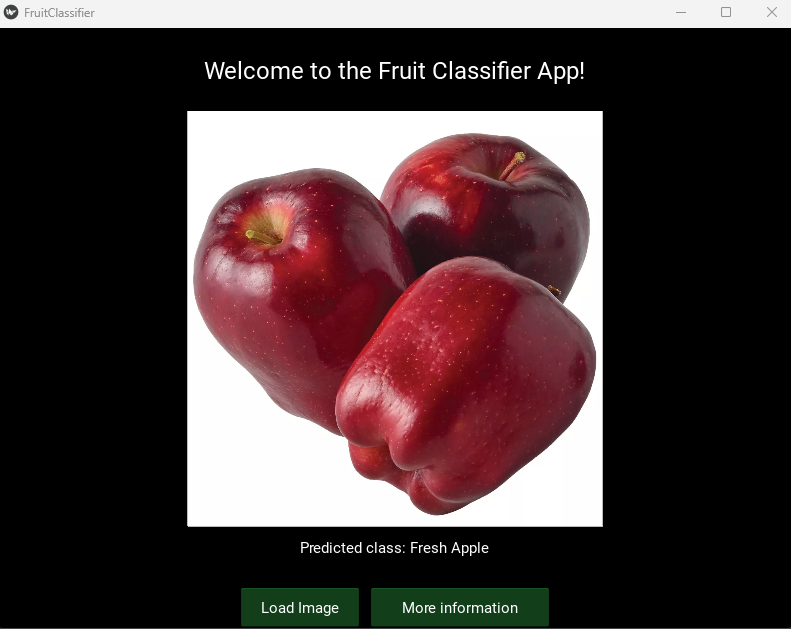
\includegraphics[width=\linewidth]{Mlayer appel1.png}
        \caption{Final Version Apple 1 Classification.}
        \label{figFA}
    \end{subfigure}
    \hfill
    \begin{subfigure}[b]{0.48\linewidth}
        \centering
        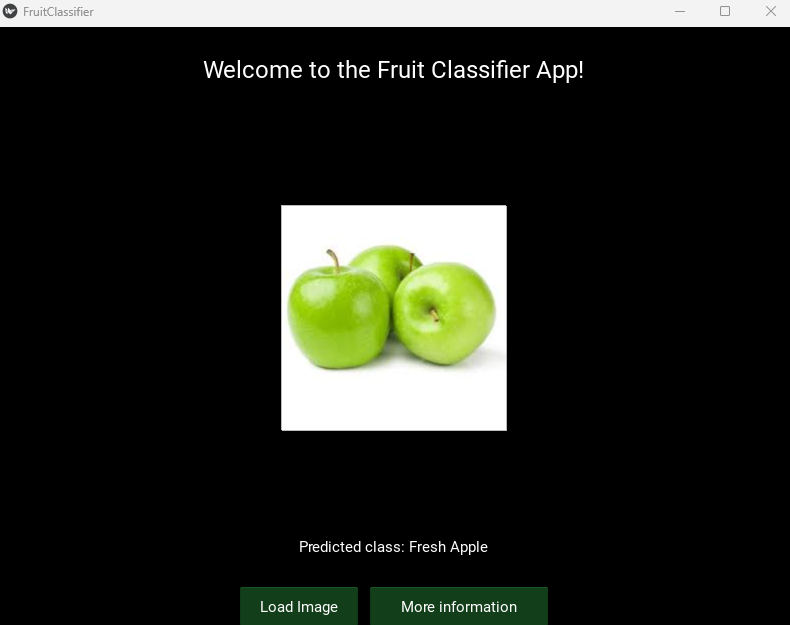
\includegraphics[width=\linewidth]{Mlayer appel2.png}
        \caption{Final Version Apple 2 Classification.}
        \label{figFB}
    \end{subfigure}
    \hfill
    \begin{subfigure}[b]{0.48\linewidth}
        \centering
        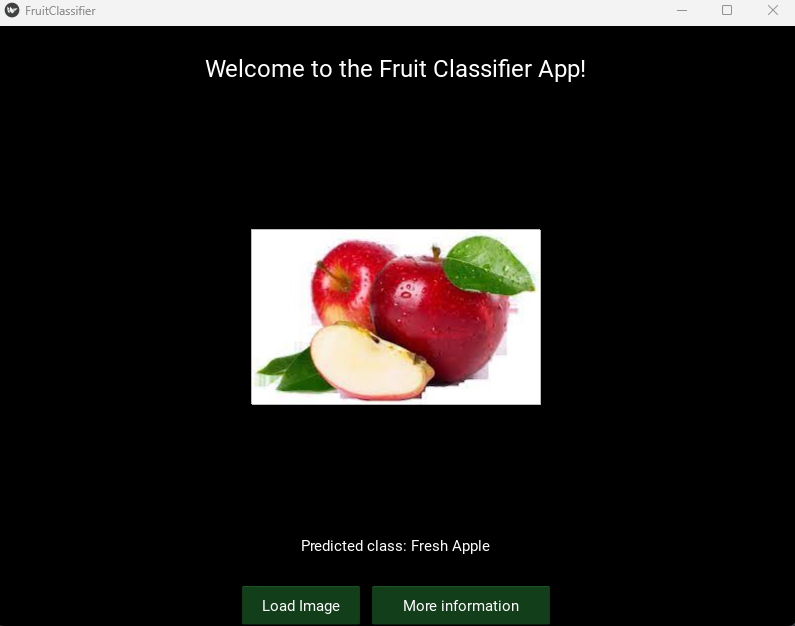
\includegraphics[width=\linewidth]{Mlayer appel3.png}
        \caption{Final Version Apple 3 Classification.}
        \label{figFB}
    \end{subfigure}
    \hfill
    \begin{subfigure}[b]{0.48\linewidth}
        \centering
        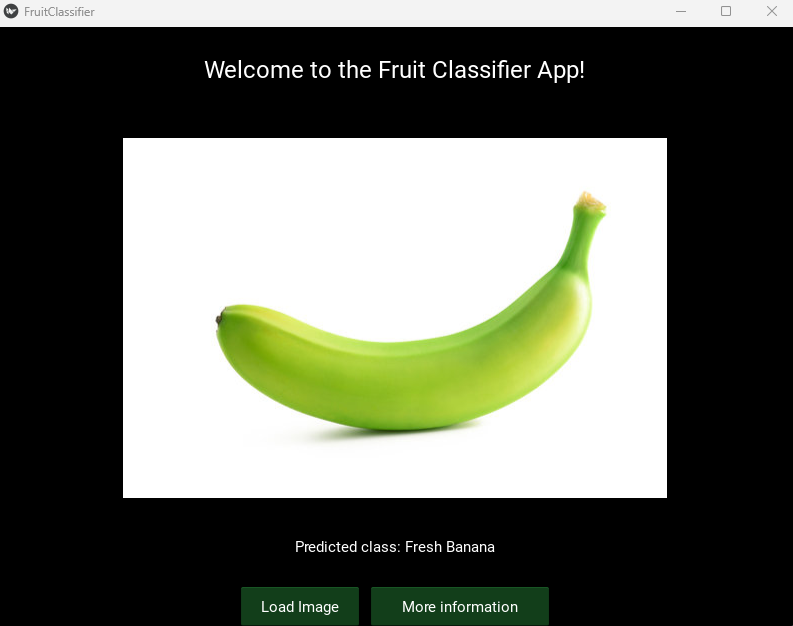
\includegraphics[width=\linewidth]{Mlayer banana1.png}
        \caption{Final Version Banana 1 Classification.}
        \label{figFA}
    \end{subfigure}
    \hfill
    \begin{subfigure}[b]{0.48\linewidth}
        \centering
        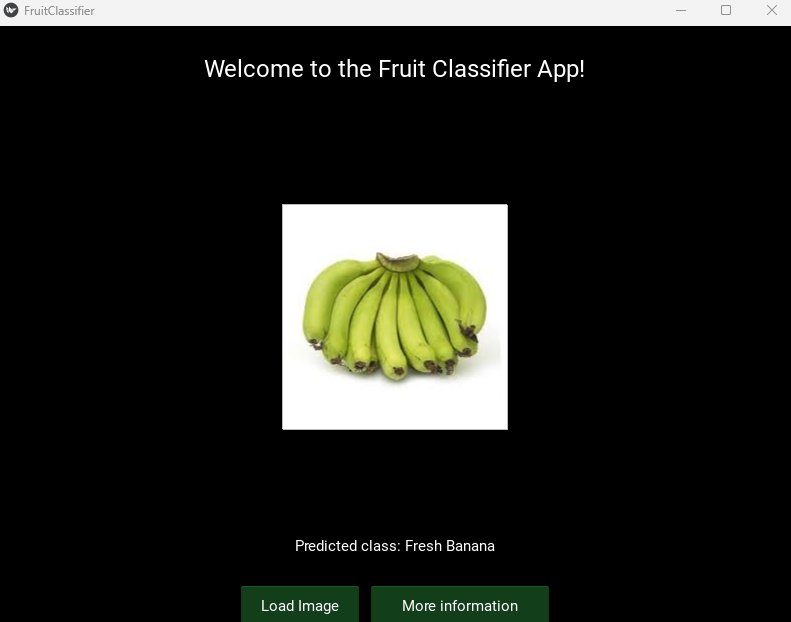
\includegraphics[width=\linewidth]{Mlayer banana2.png}
        \caption{Final Version Banana 2 Classification.}
        \label{figFB}
    \end{subfigure}
    \hfill
    \begin{subfigure}[b]{0.48\linewidth}
        \centering
        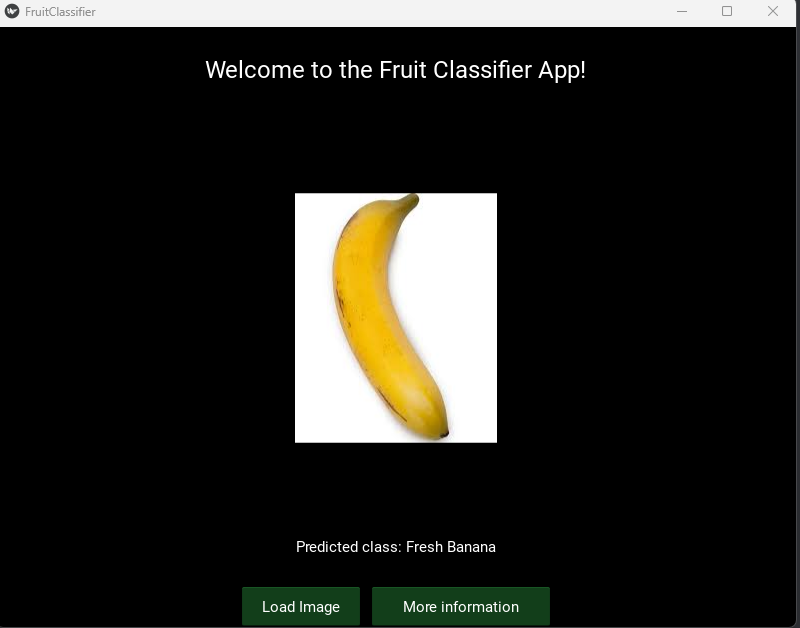
\includegraphics[width=\linewidth]{Mlayer banana3.png}
        \caption{Final Version Banana 3 Classification.}
        \label{figFB}
    \end{subfigure}
    \hfill
    \begin{subfigure}[b]{0.48\linewidth}
        \centering
        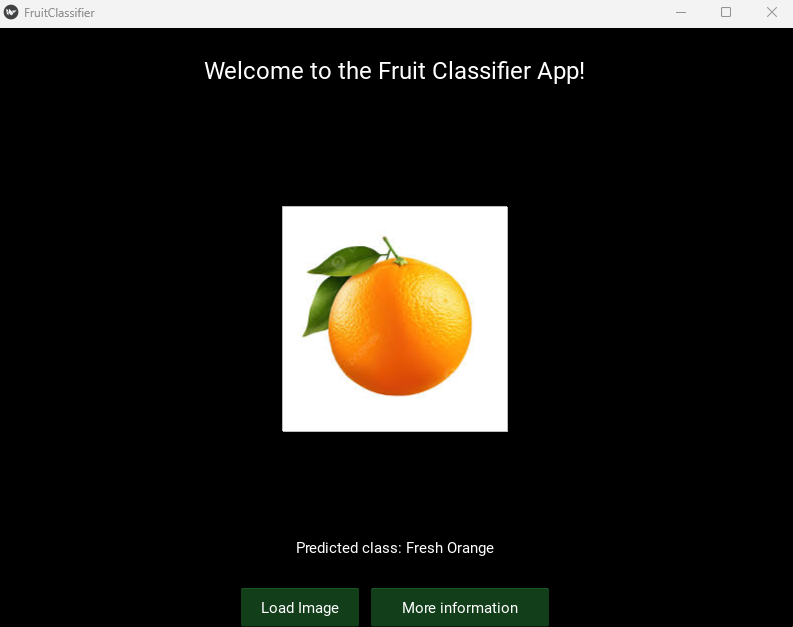
\includegraphics[width=\linewidth]{Mlayer orage1.png}
        \caption{Final Version Orange 1 Classification.}
        \label{figFA}
    \end{subfigure}
    \hfill
    \begin{subfigure}[b]{0.48\linewidth}
        \centering
        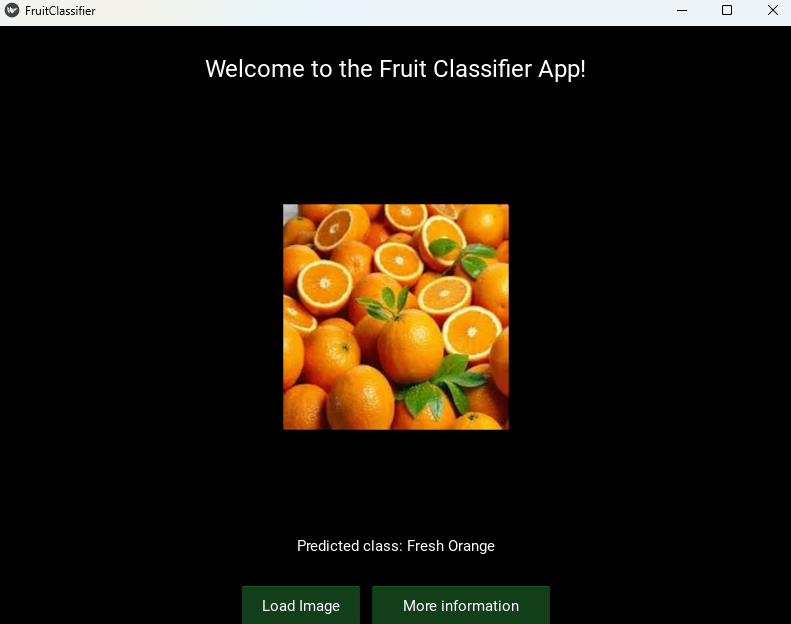
\includegraphics[width=\linewidth]{Mlayer orage2.png}
        \caption{Final Version Orange 2 Classification.}
        \label{figFB}
    \end{subfigure}
    \hfill
    \begin{subfigure}[b]{0.48\linewidth}
        \centering
        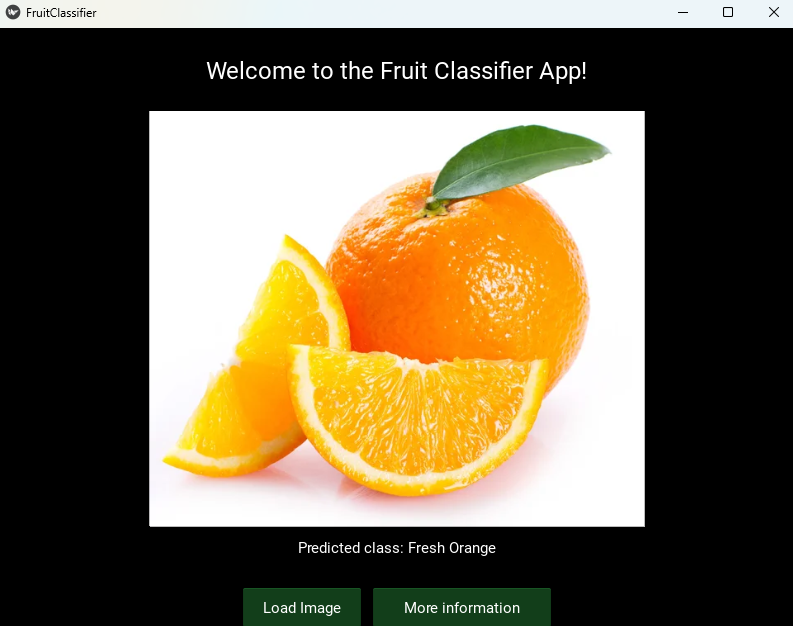
\includegraphics[width=\linewidth]{Mlayer orage3.png}
        \caption{Final Version Orange 3 Classification.}
        \label{figFB}
    \end{subfigure}
    \caption{Final Version Classification of Fresh Fruit.}
    \label{FigMF}
\end{figure}


\begin{figure}[h]
    \centering
    \begin{subfigure}[b]{0.48\linewidth}
        \centering
        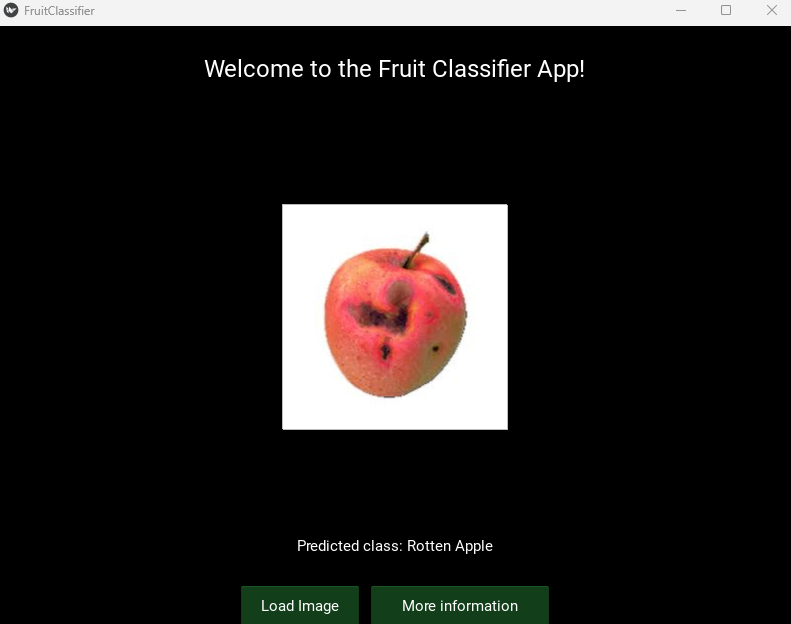
\includegraphics[width=\linewidth]{Mlayer appelR1.png}
        \caption{Final Version Apple 1 Classification.}
        \label{figFA}
    \end{subfigure}
    \hfill
    \begin{subfigure}[b]{0.48\linewidth}
        \centering
        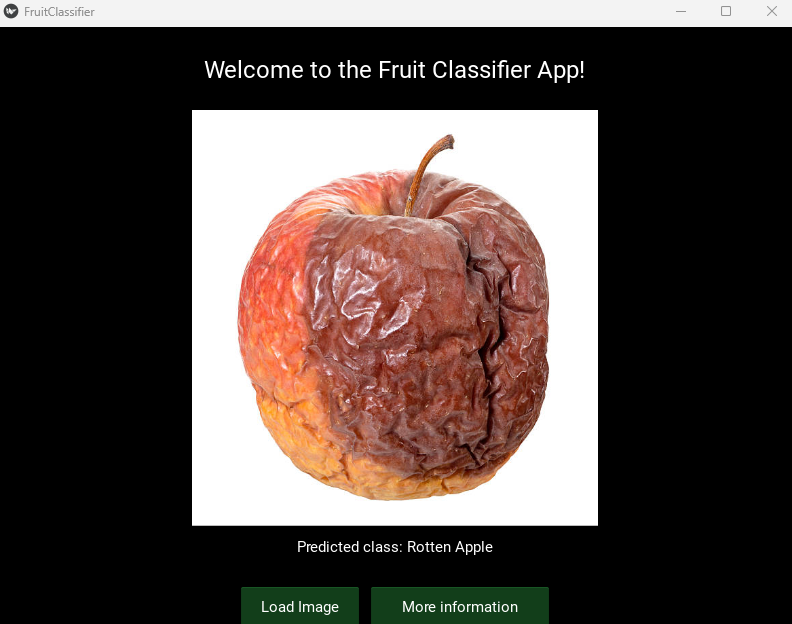
\includegraphics[width=\linewidth]{Mlayer appelR2.png}
        \caption{Final Version Apple 2 Classification.}
        \label{figFB}
    \end{subfigure}
    \hfill
    \begin{subfigure}[b]{0.48\linewidth}
        \centering
        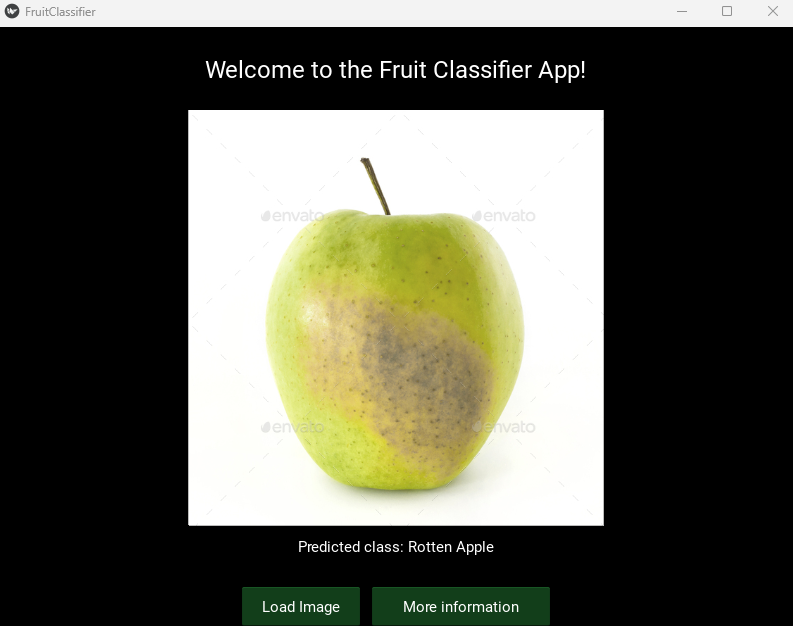
\includegraphics[width=\linewidth]{Mlayer appelR3.png}
        \caption{Final Version Apple 3 Classification.}
        \label{figFB}
    \end{subfigure}
    \hfill
    \begin{subfigure}[b]{0.48\linewidth}
        \centering
        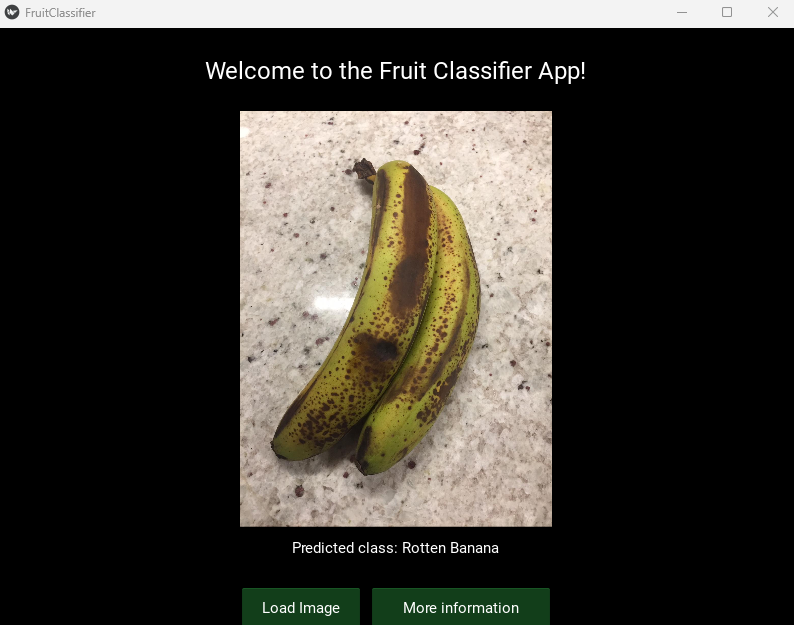
\includegraphics[width=\linewidth]{Mlayer bananaR1.png}
        \caption{Final Version Banana 1 Classification.}
        \label{figFA}
    \end{subfigure}
    \hfill
    \begin{subfigure}[b]{0.48\linewidth}
        \centering
        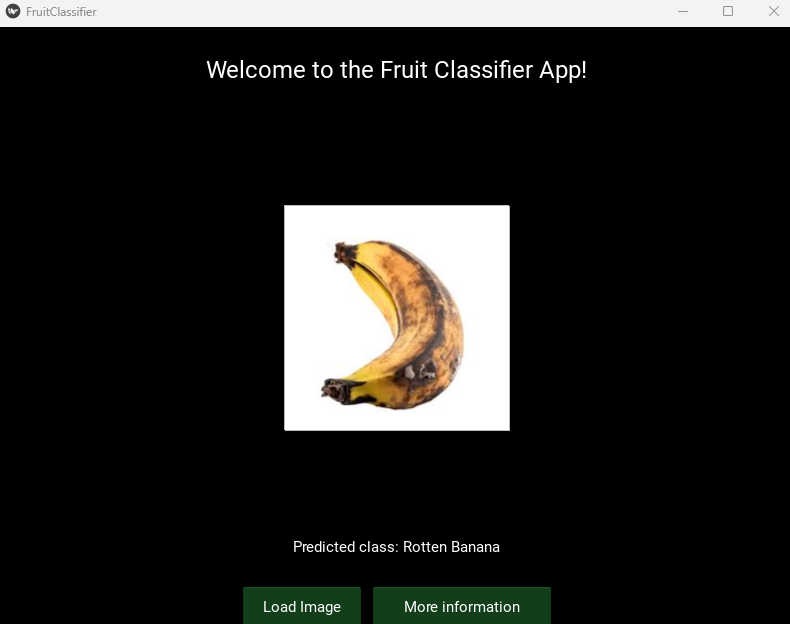
\includegraphics[width=\linewidth]{Mlayer bananaR2.png}
        \caption{Final Version Banana 2 Classification.}
        \label{figFB}
    \end{subfigure}
    \hfill
    \begin{subfigure}[b]{0.48\linewidth}
        \centering
        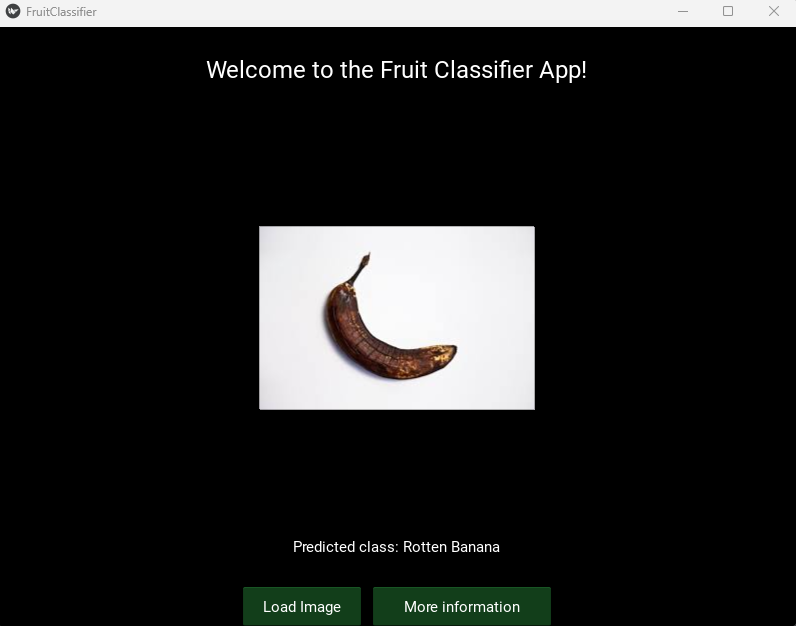
\includegraphics[width=\linewidth]{Mlayer bananaR3.png}
        \caption{Final Version Banana 3 Classification.}
        \label{figFB}
    \end{subfigure}
    \hfill
    \begin{subfigure}[b]{0.48\linewidth}
        \centering
        \includegraphics[width=\linewidth]{Mlayer orageR1.png}
        \caption{Final Version Orange 1 Classification.}
        \label{figFA}
    \end{subfigure}
    \hfill
    \begin{subfigure}[b]{0.48\linewidth}
        \centering
        \includegraphics[width=\linewidth]{Mlayer orageR2.png}
        \caption{Final Version Orange 2 Classification.}
        \label{figFB}
    \end{subfigure}
    \hfill
    \begin{subfigure}[b]{0.48\linewidth}
        \centering
        \includegraphics[width=\linewidth]{Mlayer orageR3.png}
        \caption{Final Version Orange 3 Classification.}
        \label{figFB}
    \end{subfigure}
    \caption{Final Version Classification of Rotten Fruit.}
    \label{FigMR}
\end{figure}
\clearpage

\subsection{Tabular Comparison}

\begin{figure}[h]
    \centering
    \includegraphics[width=\linewidth]{Ek wil huil.png}
    \caption{Comparison Table.}
    \label{figHuil}
\end{figure}

\begin{figure}[h]
    \centering
    \begin{subfigure}[b]{0.48\linewidth}
        \centering
        \includegraphics[width=\linewidth]{Graft1.png}
        \caption{Comparison Prediction.}
        \label{figFA}
    \end{subfigure}
    \hfill
    \begin{subfigure}[b]{0.48\linewidth}
        \centering
        \includegraphics[width=\linewidth]{Graft2.png}
        \caption{Correct Prediction.}
        \label{figFB}
    \end{subfigure}
    \caption{Graphs of different versions.}
    \label{FigGraph}
\end{figure}.

\subsection{Single Layer Vs. Multi Layer Conclusion}

The Single layer model had achieved a score of 5 out of 15. The Multi layer model had achieved a score of 15 out of 15. See Fig. \ref{figHuil} and Fig. \ref{FigGraph} for details. Both of the models were trained on a learning rate of 0.001 and 100 Epochs. The multi layer model had a patience variable implemented with a value of 10, which protected the model against overtraining. In conclusion, the multi layer model worked a lot better than the single layer model.

\section{Potential Future Development}

The following list are features that could be implemented in the future:
\begin{itemize}
    \item Use a build tool called Buildozer to package the Kivy application for iOS and Android. Building the application with Buildozer allows it to run on both platforms. We initially left this step out due to the high cost of publishing apps on the Google Play Store and the complexity of getting them approved on the Apple App Store. %BUILDOZER DIE BITCH
    \item Host the model on AWS and access it via API calls. Running the model on AWS reduces the processing load on mobile devices, as the model's processing is handled by AWS.
    \item Implement both edge detection and image colorisation. This can help to remove noise in the image and accurately classify the fruit.
\end{itemize}

\section{File List and Presentation}

\subsection{Final Written Documents}
\begin{itemize}
    \item \textit{AI Boys V2\_documentation.pdf}
    \item \textit{AI Boys V2\_final\_presentation.pptx}
\end{itemize}

\subsection{Final Coding Documents}

\subsubsection{Model Code}
\begin{itemize}
    \item \textit{Fresh\_Vs\_Rotten\_Colab.ipynb}
    \item \textit{Fresh\_Vs\_Rotten\_Desktop.ipynb}
    \item \textit{Fresh\_Vs\_Rotten\_Python.py}
\end{itemize}

\subsubsection{Mobile App}
\begin{itemize}
    \item \textit{mobile\_app.py}
\end{itemize}

\subsection{Final Models}
\begin{itemize}
    \item \textit{fruit\_classifier\_scripted.pt}
    \item \textit{fruit\_classifier.pth}
\end{itemize}


\section{Document information}
The document was created using an IEEE Overleaf LaTeX style.  We used Harvard referencing for the project's paper. The inline citation style used was Vancouver.

\section{Conclusion}

In conclusion, this paper has introduced a convolutional neural network (CNN) model and a mobile application designed to classify fresh and rotten fruits, specifically apples, bananas, and oranges. The developed CNN model leverages a structured architecture consisting of multiple convolutional layers, batch normalisation, dropout, and fully connected layers, which collectively enhance the model's ability to accurately distinguish between fresh and rotten fruits. The training process was helped  by data augmentation techniques such as random horizontal flipping and normalisation, contributing to the robustness and performance of the model.

The integration of the trained model into a mobile application demonstrates the practical applicability of this technology, providing users with a real-time tool for fruit classification. This application preprocesses user-uploaded fruit images and outputs a classification of either fresh or rotten, displaying the results alongside the input image. This model can be used to demonstrate how the automation of fruit quality assessment can be done, which streamlines sorting and grading processes in both agricultural industries and everyday usage.

By changing parameters, which included varying the number of epochs, batch sizes, convolutional layers, and the inclusion of dropout layers, was crucial in achieving an optimal balance between model accuracy and training efficiency. The final model demonstrated improved performance and reliability, though there remain certain limitations. For instance, the model's accuracy is inherently linked to the quality and diversity of the training dataset, indicating potential areas for future enhancement, such as expanding the dataset to include a broader variety of fruits and conditions.

Overall, the proposed CNN model and mobile application highlight the potential of AI-driven solutions in agricultural practices, offering a practical approach to enhance the efficiency and accuracy of fruit quality assessment. Future work could focus on extending the model's capabilities to other types of fruits, further improving the model's generalisation abilities, and integrating additional features such as user feedback mechanisms to continuously refine and update the model's accuracy in real-world scenarios.

\section*{Acknowledgment}

We would like to acknowledge Pieter Swanepoel for assisting us with the setup of the Google Colabe environment. %He is lekker.

\begin{thebibliography}{00}
    \bibitem{b10} Albardi, F., Kabir, H.D., Bhuiyan, M.M.I., Kebria, P.M., Khosravi, A. and Nahavandi, S., 2021, October. A comprehensive study on torchvision pre-trained models for fine-grained inter-species classification. In 2021 IEEE International Conference on Systems, Man, and Cybernetics (SMC) (pp. 2767-2774). IEEE.
    \bibitem{b23} Albawi, S., Mohammed, T.A. and Al-Zawi, S., 2017, August. Understanding of a convolutional neural network. In 2017 international conference on engineering and technology (ICET) (pp. 1-6). Ieee
    \bibitem{b15} Amos, D., 2020. Python gui programming with tkinter. Tersedia: https://realpython.com/python-gui-tkinter, p.71.
    \bibitem{b13} Barua, T., Doshi, R. and Hiran, K.K., 2020. Mobile Applications Development: With Python in Kivy Framework. Walter de Gruyter GmbH \& Co KG.
    \bibitem{b4} Brownlee, J., 2018. What is the Difference Between a Batch and an Epoch in a Neural Network. Machine learning mastery, 20.
    \bibitem{b17} Carneiro, T., Da Nóbrega, R.V.M., Nepomuceno, T., Bian, G.B., De Albuquerque, V.H.C. and Reboucas Filho, P.P., 2018. Performance analysis of google colaboratory as a tool for accelerating deep learning applications. Ieee Access, 6, pp.61677-61685.
    \bibitem{b28} Cenggoro, T. W., Budiarto, A., Rahutomo, R., Pardamean, B., 2018. Information system design for deep learning based plant counting automation. 2018 Indonesian Association for Pattern Recognition International Conference (INAPR), pp. 329-332.
    \bibitem{b11} Charpiat, G., Bezrukov, I., Hofmann, M., Altun, Y. and Schölkopf, B. (n.d.) 'Machine Learning Methods for Automatic Image Colorization', in Computational Photography: Methods and Applications. Pulsar Project, INRIA, Sophia-Antipolis, France, and Max Planck Institute for Biological Cybernetics, Tubingen, Germany, pp. 1-3.
    \bibitem{b22} Fajrie, N., Rohidi, T.R., Syakir, M., Syarif, I. and Priyatmojo, A.S., 2020. A study of visual impairment in the art creation process using clay. International Journal of Innovation, Creativity and Change, 11(10), pp.199-218.
    \bibitem{b6} Gu, J. et al., 2018. Recent advances in convolutional neural networks. Pattern Recognition, Volume 77, pp. 354-377.
    \bibitem{b16} Kanani, P. and Padole, M., 2019. Deep learning to detect skin cancer using google colab. International Journal of Engineering and Advanced Technology Regular Issue, 8(6), pp.2176-2183.
    \bibitem{b7} Kazuyuki, H., Daisuke, S. , Hayaru Shouno, 2015. Analysis of function of rectified linear unit used in deep learning. In: 2015 International Joint Conference on Neural Networks. s.l.:s.n., pp. 1-8.
    \bibitem{b25} Deep Learning Applications in Medical Image Analysis
    \bibitem{b2} McCandlish, S., Kaplan, J., Amodei, D. and Team, O.D., 2018. An empirical model of large-batch training. arXiv preprint arXiv:1812.06162.
    \bibitem{b18} Mohapatra, A., Yuvraj, B.K. and Shanmugasundaram, S., 2016. Physicochemical changes during ripening of red banana. International Journal of Science, Environment and Technology, 5(3), pp.1340-1348.
    \bibitem{b1} Niculescu-Mizil, A. and Caruana, R., 2007, March. Inductive transfer for Bayesian network structure learning. In Artificial intelligence and statistics (pp. 339-346). PMLR.
    \bibitem{b32} Nwankpa, C., Ijomah, W., Gachagan, A. and Marshall, S., 2018. Activation functions: Comparison of trends in practice and research for deep learning. arXiv preprint arXiv:1811.03378.
    \bibitem{b3} O'shea, K. and Nash, R., 2015. An introduction to convolutional neural networks. arXiv preprint arXiv:1511.08458.+
    \bibitem{b30} Oostwal, E., Straat, M. and Biehl, M., 2021. Hidden unit specialization in layered neural networks: ReLU vs. sigmoidal activation. Physica A: Statistical Mechanics and its Applications, 564, p.125517.
    \bibitem{b9} Paszke, A., Gross, S., Massa, F., Lerer, A., Bradbury, J., Chanan, G., Killeen, T., Lin, Z., Gimelshein, N., Antiga, L. and Desmaison, A., 2019. Pytorch: An imperative style, high-performance deep learning library. Advances in neural information processing systems, 32.
    \bibitem{b34} Pramoditha, R. (2022, September 21). How to Choose the Optimal Learning Rate for Neural Networks: Guidelines for tuning the most important neural network hyperparameter with examples. Towards Data Science. Retrieved from https://towardsdatascience.com/how-to-choose-the-optimal-learning-rate-for-neural-networks-9545d063fdb5
    \bibitem{b29} Rahutomo, R. et al., 2019. Artificial intelligence model implementation in web-based application for pineapple object counting. 2019 International Conference on Information Management and Technology (ICIMTech), Volume 1, pp. 525-530.
    \bibitem{b33} Raschka, S., Patterson, J. , Nolet, C., 2020. Machine Learning in Python:Main Developments and Technology Trends in Data Science, Machine
    Learning, and Artificial Intelligence. Information, 11(4).
    \bibitem{b20} Roushdy, M., 2006. Comparative study of edge detection algorithms applying on the grayscale noisy image using morphological filter. GVIP journal, 6(4), pp.17-23.
    \bibitem{b5} Santos, C.F.G.D. and Papa, J.P., 2022. Avoiding overfitting: A survey on regularization methods for convolutional neural networks. ACM Computing Surveys (CSUR), 54(10s), pp.1-25.
    \bibitem{b24} Shamsaldin, A. S., Fattah, P., Rashid, T. A., Al-Salihi, N. K., 2019. A study of the convolutional neural networks applications. UKH Journal of Science and Engineering, 3(2), pp. 31-40
    \bibitem{b19} Sharma, T., 2017. Various types of image noise and de-noising algorithm. International Journal of Modern Education and Computer Science, 9(5), p.50.
    \bibitem{b14} Solis, H., 2015. Kivy cookbook. Packt Publishing Ltd.
    \bibitem{b8} Teoh, T.T. and Rong, Z., 2022. Artificial intelligence with python (pp. 3-328). New York: Springer.
    \bibitem{b31} Thakur, A., 2023. ReLU vs. Sigmoid Function in Deep Neural Networks: Why ReLU is so Prevalent? What's all the fuss about using ReLU anyway? [Accessed 26 May 2024].
    \bibitem{b12} Tosi, S., 2009. Matplotlib for Python developers. Packt Publishing Ltd.
    \bibitem{b21} Yamashita R, Nishio M, Do RK, Togashi K. Convolutional neural networks: an overview and application in radiology. Insights into imaging. 2018 Aug;9:611-29.
    \bibitem{b26} Valentino, F., Cenggoro, T.W. and Pardamean, B., 2021, July. A design of deep learning experimentation for fruit freshness detection. In IOP conference series: earth and environmental science (Vol. 794, No. 1, p. 012110). IOP Publishing.
    \bibitem{b27} Wang, X., Zhao, Y. , Pourpanah, F., 2020. Recent advances in deep
    learning. Springer, Volume 11, pp. 747-750.    

\end{thebibliography}

\section*{Contribution to Project}
\begin{itemize}
    \item Bernard Swanepoel 39909476: Created the final version of the model that contained multiple conventional layer, created the Kivy mobile application, trained the model, and created presentations.
    \item Ashton du Plessis 34202676: Created the first version of the model that contained 1 conventional layer, helped with training first version of the model, did the documentation, helped with the creation of the presentation, and presented 2 out of the 3 presentations.
    \item Nico Deng 33700710: Change UI of the Kivy mobile application to be more user-friendly, helped with the documentation, helped with the creation of the presentation, and presented 1 out of the 3 presentations.
\end{itemize}

\end{document}